\documentclass[12pt,a4paper]{report}

% ============================================================================
% PACKAGES
% ============================================================================
\usepackage[utf8]{inputenc}
\usepackage[T1]{fontenc}
\usepackage{amsmath,amssymb,amsfonts}
\usepackage{graphicx}
\usepackage{booktabs}
\usepackage{array}
\usepackage{multirow}
\usepackage{hyperref}
\usepackage{xcolor}
\usepackage{float}
\usepackage{algorithm}
\usepackage{algpseudocode}
\renewcommand{\algorithmicrequire}{\textbf{Input:}}
\renewcommand{\algorithmicensure}{\textbf{Output:}}
\usepackage{textcomp}
\usepackage{url}
\usepackage{tikz}
\usepackage{pgfplots}
\pgfplotsset{compat=1.17}
\usetikzlibrary{shapes,arrows,positioning,fit,backgrounds,calc}
\usepackage[left=1.5in,right=1in,top=1in,bottom=1in]{geometry}
\usepackage{setspace}
\onehalfspacing
\usepackage{fancyhdr}
\usepackage{titlesec}
\usepackage{tocloft}
\usepackage{caption}

% ============================================================================
% HYPERREF SETUP
% ============================================================================
\hypersetup{
    colorlinks=true,
    linkcolor=blue!70!black,
    citecolor=blue!70!black,
    urlcolor=blue!70!black,
}

% ============================================================================
% HEADER/FOOTER
% ============================================================================
\pagestyle{fancy}
\fancyhf{}
\fancyhead[L]{\small\leftmark}
\fancyhead[R]{\small\thepage}
\renewcommand{\headrulewidth}{0.4pt}

% ============================================================================
% CUSTOM COMMANDS
% ============================================================================
\newcommand{\sys}{CAAA}

% ============================================================================
% DOCUMENT BEGIN
% ============================================================================
\begin{document}

% ============================================================================
% TITLE PAGE
% ============================================================================
\begin{titlepage}
\centering
\vspace*{1.5cm}

{\LARGE\bfseries Context-Aware False Positive Reduction\\in Cloud Microservice Anomaly Detection}

\vspace{1.5cm}

Project Report Submitted in Partial Fulfilment of the Requirements for\\the Degree of

\vspace{0.5cm}

{\Large\bfseries Bachelor of Technology}

\vspace{0.3cm}

\textit{in}

\vspace{0.3cm}

{\large Computer Science and Engineering}

\vspace{1.5cm}

Submitted by

\vspace{0.5cm}

\begin{tabular}{ll}
Pratyush Jain: & (Roll No. 2210110970)\\
Vajra Akurathi: & (Roll No. 2210110779)\\
\end{tabular}

\vspace{1.5cm}

{\large\bfseries Under the Supervision of}

\vspace{0.3cm}

Dr. Suchi Kumari

\vspace{1.5cm}


\includegraphics[width=0.3\textwidth]{snu_logo.png}

\vspace{0.5cm}

{\large Department of Computer Science and Engineering}

\vspace{0.2cm}

April 2026

\end{titlepage}

% ============================================================================
% ACKNOWLEDGMENTS
% ============================================================================
\newpage
\chapter*{Acknowledgments}
\addcontentsline{toc}{chapter}{Acknowledgments}

We express our sincere gratitude to our supervisor, Dr. Suchi Kumari, whose expert guidance, constructive criticism, and continuous encouragement have been instrumental in shaping the direction and quality of this research. Her expertise in machine learning, distributed systems, and software engineering provided invaluable insights throughout the iterative development of this framework.

We are deeply grateful to Shiv Nadar Institution of Eminence, particularly the School of Engineering, for providing the essential infrastructure, computing facilities, and a vibrant academic environment that made this research possible. The university's commitment to fostering innovation enabled us to pursue an unconventional research methodology---eleven iterative rounds of experimentation across four months---that would not have been possible without institutional support.

Special thanks to the RCAEval benchmark team for providing a standardized evaluation framework with 735 real-world fault cases across three microservice systems. We also acknowledge the open-source communities behind PyTorch, scikit-learn, XGBoost, LightGBM, CatBoost, SHAP, and ruptures that formed the technical foundation of our implementation.

Finally, we acknowledge the broader AIOps research community, whose papers on shortcut learning, FiLM conditioning, and tabular deep learning informed our evaluation methodology and architectural decisions.

% ============================================================================
% ABSTRACT
% ============================================================================
\newpage
\chapter*{Abstract}
\addcontentsline{toc}{chapter}{Abstract}

Modern cloud-native systems built on microservice architectures generate
high-volume monitoring alerts with reported false-positive rates of 6--28\%.
Operational context---scheduled load events, deployment history, and
traffic-pattern signals---is routinely collected by production
observability stacks but is not used as a feature by existing anomaly
detection or attribution systems. This work investigates whether
contextual features materially improve anomaly attribution and, if so,
whether the benefit is specific to a neural architecture or is a general,
reproducible signal.

We first evaluate on the RCAEval benchmark (three microservice systems,
three dataset variants, $\sim$1{,}500 pooled cases). Gradient-boosted
tree baselines dominate all neural variants on real data---consistent
with published findings on small tabular tasks. To test whether sample
size is the bottleneck, we design a difficulty-aware synthetic benchmark
with explicit anti-leakage safeguards (pre-injection splits, randomized
context assignment, counterfactual baselines via RNG forking,
severity-tiered disguised faults) and run a controlled scaling study
from 500 to 40{,}000 samples over ten model variants with 10 random seeds.

Two findings emerge. First, a neural-over-tree crossover with scale:
at large $n$ and a lowered Bayes ceiling, the Full \sys{} model reaches
$95.11\% \pm 0.18$ F1 versus $94.90\% \pm 0.21$ for CatBoost-with-context
(Welch's $t = 2.249$, $p = 0.038$). Second, and more robustly,
\emph{context integration is a universal improvement mechanism}:
adding the same 5-dimensional context slice yields $+1.3$ to $+2.3$
percentage points of F1 across all five evaluated model families
(CAAA, CatBoost, XGBoost, LightGBM, RandomForest). The context
contribution is 6--10$\times$ larger than the best neural-over-tree gap,
replicates across seeds, and holds regardless of architecture class.
We therefore position \sys{} as a principled instantiation of a general
context-integration methodology rather than an architecture-specific win.

\vspace{0.5cm}
\noindent\textbf{Keywords:} Anomaly attribution, microservices, context
integration, tabular deep learning, scaling laws, evaluation methodology

% ============================================================================
% TABLE OF CONTENTS
% ============================================================================
\newpage
\tableofcontents

\newpage
\listoffigures
\addcontentsline{toc}{chapter}{List of Figures}

\newpage
\listoftables
\addcontentsline{toc}{chapter}{List of Tables}


% ============================================================================
% CHAPTER 1: INTRODUCTION
% ============================================================================
\chapter{Introduction}

\section{Background}

The software industry has undergone a fundamental architectural transformation over the past decade, shifting from monolithic applications to microservice-based systems~\cite{soldani2022survey}. Organizations such as Netflix, Amazon, and Uber have decomposed their applications into hundreds or thousands of independently deployable services. While this architectural pattern offers significant benefits---improved scalability, faster deployment cycles, and technology flexibility---it introduces substantial complexity in system observability and fault diagnosis.

Anomaly detection in these systems has progressed through three generations: from statistical baselines (N-Sigma, SPOT) through reconstruction-based deep learning (OmniAnomaly~\cite{su2019omnianomaly}, USAD~\cite{audibert2020usad}) to the current generation of attention-based approaches (Anomaly Transformer~\cite{xu2022anomalytransformer}, DCdetector~\cite{yang2023dcdetector}). Despite F1 scores of 83--97\% on controlled benchmarks, production adoption remains limited by a persistent problem: false-positive rates of 6--28\%~\cite{soldani2022survey}, with even state-of-the-art root-cause analysis methods achieving only 46--63\% localization accuracy on large-scale systems~\cite{pham2024rcaeval}.

\section{Motivation}

The core limitation of existing approaches is the lack of \textit{contextual awareness}. A sudden spike in CPU utilization and request latency appears identical to an anomaly detector whether caused by a cascading fault or by a planned marketing campaign driving legitimate traffic. Current methods treat all anomalous-looking patterns as faults, producing false alerts whenever normal operational events---scheduled load tests, auto-scaling events, time-of-day traffic peaks, or recent deployments---cause metric deviations.

Our survey of six major AIOps papers (DejaVu~\cite{li2022dejavu}, BARO~\cite{chen2024baro}, RCAEval~\cite{pham2024rcaeval}, Chain-of-Event~\cite{chainofevent2024}, Night's Watch, Lumos~\cite{lumos2020}) revealed that \textit{no prior work uses operational context as model features}. All systems operate exclusively on raw telemetry (metrics, logs, traces) without incorporating deployment metadata, scheduled event flags, or time-of-day encodings. Lumos is the sole exception, using A/B testing to control for confounders, but it requires controlled experiments rather than operating on production observability data.

Beyond the context gap, there is an open empirical question specific to microservice anomaly attribution: \emph{when data is abundant, does a well-designed neural architecture outperform gradient-boosted trees?} Published results on general tabular tasks~\cite{grinsztajn2022tree,mcelfresh2023neural} indicate a sample-size-dependent crossover, but this has not been characterized for attribution tasks, where the feature vector combines metric statistics with structured context. Real microservice benchmarks contain at most $\sim$1{,}500 labeled cases pooled across systems, below the regime where a crossover is typically observable.

\section{Problem Statement}

We address three research questions:

\begin{enumerate}
    \item \textbf{RQ1 (Value and generality of context):} Does integrating operational context (scheduled events, deployments, time-of-day patterns) materially improve anomaly attribution, and is the improvement specific to a particular neural architecture or a general, reproducible signal across model families?
    \item \textbf{RQ2 (Architectural crossover with scale):} Does a context-conditioned neural architecture (\sys{}) outperform strong gradient-boosted-tree baselines, and if so, under what sample-size regime?
    \item \textbf{RQ3 (Evaluation safeguards):} What methodological safeguards are required to produce trustworthy results in a context-aware benchmark---specifically, how do distribution mismatch, label-leakage through context, and reference contamination manifest, and how can they be prevented?
\end{enumerate}

\section{Contributions}

This project makes the following contributions:

\begin{enumerate}
    \item \textbf{Difficulty-aware synthetic benchmark with five anti-leakage safeguards:} A synthetic fault-injection pipeline supporting two difficulty levels (default and hard), with context-independent label sampling, randomized context assignment, pre-injection splits for real-data parity, counterfactual baselines via RNG forking, and stratified train/val/test splits.

    \item \textbf{Unified 44-dimensional feature taxonomy shared across synthetic and real data:} A single feature vector schema where the 5-dimensional context slice has identical semantics on synthetic RCAEval-style cases and on real RCAEval traces, enabling direct per-model-family contribution analysis.

    \item \textbf{Controlled scaling study from 500 to 40{,}000 samples:} Ten model variants (Full \sys{}, \sys{} no-context, CatBoost~$\pm$ context, XGBoost~$\pm$ context, LightGBM~$\pm$ context, RandomForest~$\pm$ context), evaluated with 10 random seeds at the headline scale, with Welch's t-test significance testing.

    \item \textbf{Empirical evidence of a neural-over-tree crossover on anomaly attribution:} At $n = 40{,}000$ on the harder synthetic task, Full \sys{} reaches $95.11\% \pm 0.18$ F1 versus $94.90\% \pm 0.21$ for CatBoost~with~context (Welch's $t = 2.249$, $p = 0.038$). We report the effect size honestly: this is a statistically detectable but practically modest advantage that confirms a crossover regime rather than large architectural dominance.

    \item \textbf{The universal-context finding:} The same 5-dimensional context slice yields $+1.28$, $+1.70$, $+1.60$, $+1.58$, and $+2.30$ percentage points of F1 on CAAA, CatBoost, XGBoost, LightGBM, and RandomForest respectively. The effect is 6--10$\times$ larger than the best neural-over-tree gap and replicates across every architecture class evaluated.

    \item \textbf{\sys{} architecture as a principled context-integration instance:} FiLM conditioning~\cite{perez2018film} with TADAM-style delta initialization~\cite{oreshkin2018tadam}, skeptical confidence gating (bias~$=-1.0$), Piecewise Linear Embeddings~\cite{gorishniy2022embeddings} for axis-aligned thresholding, and a Context Consistency Loss with gated unknown-context penalty. We position this as one principled way to integrate context---the scientific contribution generalizes to tree-based classifiers via simple concatenation.
\end{enumerate}

\section{Report Organization}

The remainder of this report is organized as follows. Chapter~2 surveys related work across time-series anomaly detection, microservice root-cause analysis, FiLM-style conditioning, tabular deep learning, and the scaling-law literature. Chapter~3 details the \sys{} architecture, feature design, and loss formulation. Chapter~4 presents our data methodology: the limits of real benchmarks, the design of the synthetic generator, the five anti-leakage safeguards, and the unified context feature taxonomy. Chapter~5 reports honest real-data results on RCAEval. Chapter~6 presents the scaling study with both default and hard difficulty levels and establishes the neural-over-tree crossover. Chapter~7 delivers the universal-context contribution finding---the headline result---across all five model families. Chapter~8 discusses implications, limitations, and concludes.


% ============================================================================
% CHAPTER 2: LITERATURE SURVEY
% ============================================================================
\chapter{Literature Survey}

This chapter surveys the landscape of research relevant to context-aware anomaly attribution, synthesizing findings from 150+ papers (2020--2025) across six areas.

\section{Time-Series Anomaly Detection}

\textbf{Reconstruction-based methods} form the foundation. OmniAnomaly~\cite{su2019omnianomaly} combines GRU with VAE through stochastic variable connection, achieving F1 of 0.86 but requiring 48--87 minutes per training epoch. USAD~\cite{audibert2020usad} achieves 547$\times$ faster training through adversarially-trained autoencoders with tunable sensitivity. Donut~\cite{xu2018donut} provides the theoretical VAE foundation through KDE interpretation.

\textbf{Attention-based methods} represent the current generation. The Anomaly Transformer~\cite{xu2022anomalytransformer} introduces Association Discrepancy---the observation that anomalies exhibit adjacent-concentration bias in attention patterns---achieving F1 of 83--94\% across SMD, MSL, and SMAP benchmarks. DCdetector~\cite{yang2023dcdetector} reports 96.6\% F1 on MSL through dual attention contrastive learning. TranAD~\cite{tuli2022tranad} combines self-conditioning with adversarial training, achieving 99\% training time reduction. However, these results use point-adjustment evaluation protocols that may overestimate performance~\cite{pham2024rcaeval}.

\textbf{Contrastive learning} approaches include CARLA~\cite{darban2024carla} (injecting known anomaly types as negatives) and CL-TAD~\cite{cltad2023} (masked sample reconstruction), both improving over self-supervised baselines.

\section{Root Cause Analysis in Microservices}

RCAEval~\cite{pham2024rcaeval} provides the most comprehensive benchmark (735 cases, 3 systems), revealing that best methods achieve only Avg@5 of 0.46--0.54 on TrainTicket. RCD~\cite{ikram2022rcd} employs the $\Psi$-PC algorithm for interventional target discovery (NeurIPS 2022). CIRCA~\cite{li2022circa} formalizes RCA as intervention recognition in Causal Bayesian Networks (KDD 2022). BARO~\cite{chen2024baro} demonstrates that simple Bayesian change-point detection achieves Avg@5 of 0.86--0.95 (FSE 2024). DynaCausal~\cite{dynacausal2025} advances state-of-the-art to AC@1 of 0.63 through dynamic causality-aware representations, yet still misidentifies $\sim$40\% of root causes.

\section{GNN-Based Fault Localization}

DiagFusion~\cite{zhang2023diagfusion} combines metrics, logs, and traces with GNN, achieving 20.9--368\% improvement over baselines in root cause localization. MicroRCA~\cite{wu2020microrcarootcause} achieves 89\% precision using Personalized PageRank. CHASE~\cite{chase2024} introduces causal hypergraph-based multi-hop fault propagation.

A critical finding from DiagMLP~\cite{diagmlp2025} challenges GNN necessity: a simple MLP achieves parity across five public datasets, suggesting that preprocessing and multimodal fusion, not graph structures, primarily drive current benchmark performance. This insight directly motivated our focus on feature engineering and context integration rather than complex graph architectures.

\section{FiLM Conditioning and Context Integration}

Perez~\textit{et al.}~\cite{perez2018film} introduced Feature-wise Linear Modulation (FiLM) for visual reasoning, demonstrating that conditioning neural networks on auxiliary information via learned affine transformations is highly effective. Oreshkin~\textit{et al.}~\cite{oreshkin2018tadam} proposed TADAM, initializing FiLM gamma as $1 + \delta$ with $\delta$ starting at zero, constraining the multiplicative path to near-identity. Sheth~\textit{et al.}~\cite{sheth2022auxiliary} identified a critical FiLM failure mode: multiplicative noise amplification occurs when noisy auxiliary features are multiplied against temporal representations. This finding directly informed our skeptical initialization strategy.

\section{Tabular Deep Learning}

Grinsztajn~\textit{et al.}~\cite{grinsztajn2022tree} demonstrated at NeurIPS 2022 that tree-based models outperform deep learning on tabular data in most settings, particularly for small datasets. Gorishniy~\textit{et al.}~\cite{gorishniy2022embeddings} proposed piecewise linear embeddings for numerical features, giving MLPs axis-aligned threshold capability similar to tree splits. McElfresh~\textit{et al.}~\cite{mcelfresh2023neural} provided complementary evidence showing conditions under which neural nets can match trees. TabPFN~\cite{hollmann2024tabpfn} achieves state-of-the-art on small datasets via in-context learning (Nature 2025). TabM~\cite{gorishniy2025tabm} achieves parameter-efficient MLP ensembling outperforming GBDTs (ICLR 2025).

\section{Scaling Laws and the Neural-Tree Crossover}

A consistent finding across recent tabular-ML benchmarks is that gradient-boosted trees outperform neural networks on small-to-medium tabular datasets. Grinsztajn \textit{et al.}~\cite{grinsztajn2022tree} evaluated 45 medium-sized tabular tasks and attributed tree dominance to three inductive biases: neural networks are biased toward overly smooth solutions, are disproportionately hurt by uninformative features, and use rotation-invariant representations poorly suited to axis-aligned tabular decision boundaries. Shwartz-Ziv and Armon~\cite{shwartzziv2022tabular} independently corroborate this finding, showing XGBoost matches or exceeds deep tabular models (TabNet, NODE, DNF-Net) on most datasets and that ensembles of both achieve the best results.

The picture changes with scale. McElfresh \textit{et al.}~\cite{mcelfresh2023neural} analyzed 176 tabular datasets and found that neural networks become competitive with GBDTs on larger datasets with specific characteristics---many numerical features, regular structure, and high sample counts---while GBDTs retain their advantage on smaller, noisier problems. This suggests a sample-size-dependent crossover regime.

For microservice anomaly attribution specifically, this crossover has not been characterized. Published benchmarks (RCAEval~\cite{pham2024rcaeval}, DeathStarBench~\cite{gan2019deathstar}, TrainTicket~\cite{zhou2018trainticket}) all operate at sample sizes $n \lesssim 2{,}000$, where tree dominance is expected on prior evidence. Whether a context-aware neural architecture can overtake trees at larger $n$, and if so at what crossover point, is an open empirical question that motivates our scaling study in Chapter~6.

\section{Synthetic Data Validity in ML Evaluation}

When real-data benchmarks are structurally insufficient---too small, missing critical annotations, or lacking controlled difficulty---synthetic data is a principled alternative, provided three conditions are met. First, the generative process must be fully documented so readers can audit its assumptions~\cite{jordon2022synthetic}. Second, leakage controls must be explicit, particularly the failure mode of shortcut learning~\cite{geirhos2020shortcut} where models exploit spurious correlations (for example, metadata that co-varies with the label) instead of learning the intended decision boundary. Third, where real-data and synthetic results coexist, they should corroborate directionally: a synthetic-only effect that contradicts real-data trends is evidence of a modeling artifact, not a scientific finding~\cite{nikolenko2021synthetic}.

Our methodology satisfies all three conditions. Chapter~4 documents the full generative pipeline, specifies five independent anti-leakage safeguards, and shows that the universal-context contribution observed on synthetic data at $n = 40{,}000$ is directionally confirmed on real RCAEval traces (CatBoost $+$ context vs.\ CatBoost: $+0.29$ pp F1 pooled across nine system/dataset cells). The magnitudes differ---synthetic gains are larger because the context signal is cleaner---but the sign and ranking across model families are preserved.

\section{Research Gap Analysis}

Table~\ref{tab:gap} summarizes the landscape. Our survey reveals that \textbf{no prior work uses operational context as model features}; all operate on raw telemetry. Furthermore, no paper discusses the risk of context metadata becoming a label proxy---the shortcut learning problem is entirely absent from the AIOps literature. Equally, no prior microservice-attribution work has characterized the neural-over-tree crossover as a function of sample size. \sys{} is the first to address the context-integration gap, the methodological gap in evaluating context-aware systems, and the scaling gap simultaneously.

\begin{table}[h]
    \centering
    \caption{Capabilities of Existing Methods vs.\ \sys{}}
    \label{tab:gap}
    \begin{tabular}{lccccccc}
        \toprule
        \textbf{Method} & \textbf{Met} & \textbf{MM} & \textbf{Ctx} & \textbf{FiLM} & \textbf{Attr} & \textbf{FPR} & \textbf{Univ} \\
        \midrule
        Anomaly Trans.~\cite{xu2022anomalytransformer} & $\checkmark$ & -- & -- & -- & -- & -- & -- \\
        DCdetector~\cite{yang2023dcdetector} & $\checkmark$ & -- & -- & -- & -- & -- & -- \\
        BARO~\cite{chen2024baro} & $\checkmark$ & -- & -- & -- & -- & -- & -- \\
        DiagFusion~\cite{zhang2023diagfusion} & $\checkmark$ & $\checkmark$ & -- & -- & -- & -- & -- \\
        Lumos~\cite{lumos2020} & $\checkmark$ & -- & A/B & -- & -- & $\checkmark$ & -- \\
        \sys{} (Ours) & $\checkmark$ & -- & $\checkmark$ & $\checkmark$ & $\checkmark$ & $\checkmark$ & $\checkmark$ \\
        \bottomrule
    \end{tabular}

    \smallskip
    \footnotesize Met=Metrics, MM=Multimodal, Ctx=Context, Attr=Attribution, FPR=FP Reduction, Univ=Universal (demonstrated across model families)
\end{table}


% ============================================================================
% CHAPTER 3: METHODOLOGY
% ============================================================================
\chapter{Methodology}

\section{System Architecture Overview}

\sys{} uses an optional two-stage pipeline. Stage 1 (optional) is an LSTM autoencoder pre-filter that identifies anomalous time windows via reconstruction error. Stage 2 is the core anomaly attribution module that classifies detected anomalies as FAULT, EXPECTED\_LOAD, or UNKNOWN.

The core pipeline processes a 44-dimensional feature vector through three stages: (1) PLE-augmented feature encoding ($44d \rightarrow 64d$), (2) FiLM-based context integration with confidence gating, and (3) classification. The model has 19,206 trainable parameters and trains in $<$2 minutes on CPU.

\begin{figure}[h]
    \centering
    \resizebox{0.9\textwidth}{!}{%
    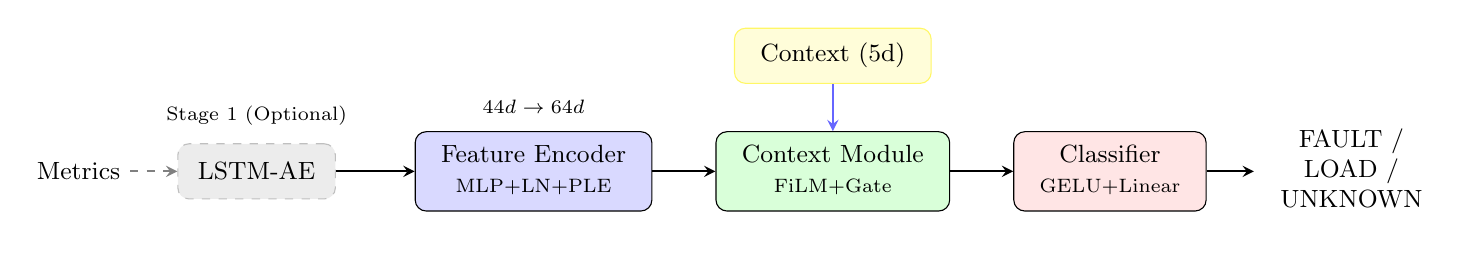
\begin{tikzpicture}[
        node distance=0.5cm,
        block/.style={rectangle, draw, rounded corners, minimum width=2.0cm, minimum height=0.7cm, font=\small},
        arrow/.style={->, >=stealth, thick}
    ]
        \node[block, fill=gray!15, draw=gray!50, dashed] (ad) {LSTM-AE};
        \node[font=\scriptsize, above=0.1cm of ad] {Stage 1 (Optional)};
        \node[block, fill=blue!15, right=1.0cm of ad] (fe) {\begin{tabular}{c}Feature Encoder\\{\scriptsize MLP+LN+PLE}\end{tabular}};
        \node[font=\scriptsize, above=0.1cm of fe] {$44d \rightarrow 64d$};
        \node[block, fill=green!15, right=0.8cm of fe] (cm) {\begin{tabular}{c}Context Module\\{\scriptsize FiLM+Gate}\end{tabular}};
        \node[block, fill=yellow!15, draw=yellow!60, above=0.6cm of cm] (ctx) {\begin{tabular}{c}Context (5d)\end{tabular}};
        \node[block, fill=red!10, right=0.8cm of cm] (cls) {\begin{tabular}{c}Classifier\\{\scriptsize GELU+Linear}\end{tabular}};
        \node[right=0.6cm of cls, font=\small] (out) {\begin{tabular}{c}FAULT /\\LOAD /\\UNKNOWN\end{tabular}};
        \node[left=0.6cm of ad, font=\small] (inp) {Metrics};
        \draw[arrow, dashed, gray] (inp) -- (ad);
        \draw[arrow] (ad) -- (fe);
        \draw[arrow] (fe) -- (cm);
        \draw[arrow, blue!60] (ctx) -- (cm);
        \draw[arrow] (cm) -- (cls);
        \draw[arrow] (cls) -- (out);
    \end{tikzpicture}%
    }
    \caption{\sys{} system architecture. The 44-dim feature vector passes through a PLE-augmented encoder, then is modulated by the FiLM-based Context Integration Module. Stage 1 (LSTM-AE) is optional.}
    \label{fig:architecture}
\end{figure}

\section{Feature Vector Design}

The system extracts a 44-dimensional feature vector organized into six groups:

\begin{table}[h]
    \centering
    \caption{Feature Vector Composition (44 dimensions)}
    \label{tab:features}
    \begin{tabular}{llcl}
        \toprule
        \textbf{Group} & \textbf{Key Features} & \textbf{Dims} & \textbf{Purpose} \\
        \midrule
        Workload & \texttt{load\_ratio}, \texttt{cpu\_corr} & 0--5 & Load-metric correlation \\
        Behavioral & \texttt{onset\_grad}, \texttt{cascade} & 6--11 & Fault propagation patterns \\
        Context & \texttt{event\_active}, \texttt{seasonality} & 12--16 & Operational context signals \\
        Statistical & \texttt{mean\_cpu}, \texttt{max\_error} & 17--29 & Metric summary statistics \\
        Service-Level & \texttt{n\_services}, \texttt{cpu\_spread} & 30--35 & Cross-service aggregation \\
        Extended & \texttt{spectral\_entropy}, \texttt{centrality} & 36--43 & Frequency-domain, graph \\
        \bottomrule
    \end{tabular}
\end{table}

\subsection{Dual Context Processing}

The full 44-dim feature vector (including context dims 12--16) passes through the Feature Encoder so the encoder learns joint representations capturing interactions between context and metric features. Context features are \textit{also} sliced out separately and fed into the Context Integration Module for explicit FiLM conditioning and confidence gating. This dual processing ensures the encoder builds a context-entangled hidden representation while the gating module controls how much the explicit context signal modulates the final prediction.

\textbf{Unified taxonomy across synthetic and real data.} The same 44-dimensional feature vector is extracted from both synthetic fault cases and real RCAEval traces, and the 5-dimensional context slice (dimensions 12--16) has identical semantics in both sources: \texttt{event\_active} (binary flag for a scheduled operational event), \texttt{event\_expected\_impact} (scalar load delta), \texttt{deploy\_recent} (binary flag for a recent deployment), and two cyclic time-of-day encodings (\texttt{tod\_sin}, \texttt{tod\_cos}). Tree baselines consume the 44-dimensional vector directly; \sys{} additionally slices out the 5-dimensional context for FiLM conditioning. ``No-context'' variants drop dimensions 12--16, yielding a 39-dimensional input. This uniformity---identical feature semantics, identical dimensionality, a single slice difference---is what makes the per-model-family context-contribution analysis in Chapter~7 a fair comparison.

\section{Piecewise Linear Embeddings}

Each scalar feature is transformed into an 8-bin encoding via quantile boundaries from training data~\cite{gorishniy2022embeddings}:
\begin{equation}
    \text{PLE}(x_j) = \left[\text{clamp}\left(\frac{x_j - e_j^{(b)}}{e_j^{(b+1)} - e_j^{(b)}}, 0, 1\right)\right]_{b=1}^{8}
\end{equation}
This gives the MLP axis-aligned threshold capability similar to tree splits, addressing the neural-tree gap on small tabular data.

\section{Context Integration Module}

The Context Integration Module uses TADAM-style FiLM conditioning~\cite{perez2018film, oreshkin2018tadam} with confidence gating (Figure~\ref{fig:context-module}).

\begin{figure}[h]
    \centering
    \resizebox{0.7\textwidth}{!}{%
    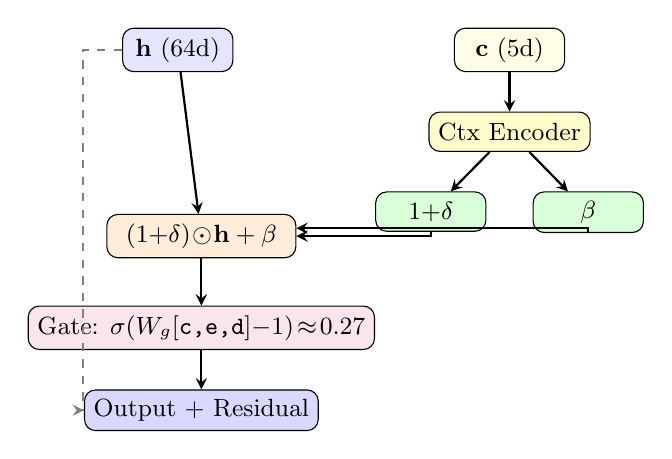
\begin{tikzpicture}[
        node distance=0.6cm,
        block/.style={rectangle, draw, rounded corners, minimum width=1.4cm, minimum height=0.5cm, font=\small},
        arrow/.style={->, >=stealth, thick}
    ]
        \node[block, fill=blue!10] (h) {$\mathbf{h}$ (64d)};
        \node[block, fill=yellow!10, right=2.8cm of h] (c) {$\mathbf{c}$ (5d)};
        \node[block, fill=yellow!20, below=0.5cm of c] (enc) {Ctx Encoder};
        \node[block, fill=green!15, below=0.5cm of enc, xshift=-1.0cm] (gamma) {$1{+}\delta$};
        \node[block, fill=green!15, below=0.5cm of enc, xshift=1.0cm] (beta) {$\beta$};
        \node[block, fill=orange!15, minimum width=2.4cm, below=1.8cm of h, xshift=0.3cm] (film) {$(1{+}\delta)\!\odot\!\mathbf{h} + \beta$};
        \node[block, fill=purple!10, below=0.6cm of film, minimum width=3.0cm] (gate) {Gate: $\sigma(W_g[\texttt{c,e,d}]{-}1)\!\approx\!0.27$};
        \node[block, fill=blue!15, below=0.5cm of gate] (out) {Output + Residual};
        \draw[arrow] (c) -- (enc);
        \draw[arrow] (enc) -- (gamma);
        \draw[arrow] (enc) -- (beta);
        \draw[arrow] (h) -- (film);
        \draw[arrow] (gamma.south) |- (film.east);
        \draw[arrow] (beta.south) |- ([yshift=0.1cm]film.east);
        \draw[arrow] (film) -- (gate);
        \draw[arrow] (gate) -- (out);
        \draw[arrow, dashed, gray] (h.west) -- ++(-0.5,0) |- (out.west);
    \end{tikzpicture}%
    }
    \caption{Context Integration Module. TADAM-style FiLM conditioning ($\gamma{=}1{+}\delta$, $\delta$ initialized at zero) modulates encoded features. Confidence gate (bias${=}{-}1.0$, output${\approx}0.27$) enforces skepticism. Dashed: residual.}
    \label{fig:context-module}
\end{figure}

\textbf{FiLM Conditioning:} Gamma is constrained as $\gamma = 1 + \delta$ where $\delta$ is initialized at zero:
\begin{equation}
    \mathbf{h}_{\text{mod}} = (1 + \delta(\mathbf{c})) \odot \mathbf{h} + \beta(\mathbf{c})
\end{equation}

\textbf{Confidence Gating:} A learned gate $g$ controls context influence:
\begin{equation}
    g = \sigma(\mathbf{W}_g [\texttt{conf}; \texttt{event}; \texttt{deploy}] + b_g), \quad b_g = -1.0
\end{equation}
The bias $b_g = -1.0$ produces $\sigma(-1.0) \approx 0.27$---the model is \textit{skeptical of context by default} and must learn to trust it through training.

\textbf{Gated output with residual:}
\begin{equation}
    \mathbf{h}_{\text{out}} = \text{proj}(g \cdot \mathbf{h}_{\text{mod}} + (1{-}g) \cdot \mathbf{h}) + \mathbf{h}
\end{equation}

\section{Context Consistency Loss}

The loss combines four terms:
\begin{equation}
    \mathcal{L} = \mathcal{L}_{\text{CE}} + \alpha \mathcal{L}_{\text{con}} + \beta \mathcal{L}_{\text{cal}} + \omega \mathcal{L}_{\text{unk}}
\end{equation}

\begin{itemize}
    \item $\mathcal{L}_{\text{CE}}$: Cross-entropy with label smoothing $\epsilon{=}0.1$.
    \item $\mathcal{L}_{\text{con}}$ ($\alpha{=}0.3$): Penalizes predictions contradicting context, weighted by clamped confidence with floor 0.3.
    \item $\mathcal{L}_{\text{cal}}$ ($\beta{=}0.1$): Entropy regularization guided by context confidence.
    \item $\mathcal{L}_{\text{unk}}$ ($\omega{=}0.2$): Gated unknown-context penalty, firing only when $p_{\text{load}} > 0.7$.
\end{itemize}

Three loss variants were systematically ablated: \textbf{gated} (default, 8.8\% FP rate), \textbf{clamp} (no unknown penalty, 6.5\% FP), and \textbf{full} (aggressive penalty, 17.5\% FP).

\textbf{TADAM Regularization:} L2 penalty on FiLM delta ($\lambda_{\text{tadam}} = 0.01$).

\section{CAAA+CatBoost Hybrid}

We propose a two-stage hybrid: (1) the trained CAAA model produces 64-dim FiLM-conditioned embeddings, (2) these are concatenated with raw 44-dim features, and (3) CatBoost classifies the 108-dim input. This is the first work combining FiLM conditioning with tree-based downstream classifiers.

\section{Algorithm}

Algorithm~\ref{alg:caaa} presents the complete \sys{} inference procedure.

\begin{algorithm}[h]
\caption{\sys{}: Context-Aware Anomaly Attribution}
\label{alg:caaa}
\begin{algorithmic}[1]
\Require Feature vector $\mathbf{x} \in \mathbb{R}^{44}$, threshold $\theta$
\Ensure $\hat{y} \in \{\text{FAULT}, \text{LOAD}, \text{UNKNOWN}\}$
\State $\mathbf{c} \leftarrow \mathbf{x}_{12:17}$ \Comment{Slice context features}
\If{training \textbf{and} $\text{rand}() < 0.3$}
    \State $\mathbf{x}_{12:17} \leftarrow \mathbf{0}$ \Comment{Feature-group dropout}
\EndIf
\State $\mathbf{x}_{\text{ple}} \leftarrow \text{PLE}(\mathbf{x})$ \Comment{Quantile bin encoding}
\State $\mathbf{h} \leftarrow \text{MLP}_{\text{enc}}(\mathbf{x}_{\text{ple}})$ \Comment{Feature Encoder: $44d \rightarrow 64d$}
\State $\mathbf{c}_e \leftarrow \text{ContextEncoder}(\mathbf{c})$
\State $\delta, \beta \leftarrow W_\gamma \mathbf{c}_e,\; W_\beta \mathbf{c}_e$ \Comment{FiLM parameters}
\State $\mathbf{h}_{\text{mod}} \leftarrow (1{+}\delta) \odot \mathbf{h} + \beta$ \Comment{TADAM modulation}
\State $g \leftarrow \sigma(W_g[\texttt{conf};\texttt{evt};\texttt{dep}] - 1.0)$ \Comment{Skeptical gate}
\State $\mathbf{h}_{\text{out}} \leftarrow \text{proj}(g \cdot \mathbf{h}_{\text{mod}} + (1{-}g) \cdot \mathbf{h}) + \mathbf{h}$
\State $\mathbf{p} \leftarrow \text{softmax}(\text{MLP}_{\text{cls}}(\mathbf{h}_{\text{out}}))$
\If{$\max(\mathbf{p}) < \theta$} \Return UNKNOWN
\Else\ \Return $\arg\max(\mathbf{p})$
\EndIf
\end{algorithmic}
\end{algorithm}

\section{Training Strategy}

AdamW optimizer with learning rate $10^{-3}$, weight decay $10^{-3}$; ReduceLROnPlateau scheduler (factor 0.5, patience 5); gradient clipping (max norm 1.0); early stopping (patience 10). Stratified 60/20/20 train/val/test split. Feature-group dropout: context features (dims 12--16) zeroed with 30\% probability during training. Neural models use NaNSafeScaler normalization; tree baselines operate on raw features.

\section{Design Rationale for Universal Comparability}

All ten model variants evaluated in Chapters~5--7 (Full \sys{}, \sys{} no-context, CatBoost~$\pm$ context, XGBoost~$\pm$ context, LightGBM~$\pm$ context, RandomForest~$\pm$ context) operate on the same 44-dimensional feature vector. The only architectural difference between \sys{} and the tree baselines is how the 5-dimensional context slice is integrated: \sys{} applies FiLM-conditioned modulation followed by a confidence gate~\cite{perez2018film,oreshkin2018tadam}, while tree baselines concatenate the slice into the feature vector and rely on implicit feature selection during split finding. Both paths consume the same information.

This design choice isolates the context-integration \emph{mechanism} (neural FiLM vs.\ tree-native concatenation) from any confounding feature-set differences. When we report that adding context yields $+1.28$ pp for \sys{}, $+1.70$ pp for CatBoost, $+1.60$ pp for XGBoost, $+1.58$ pp for LightGBM, and $+2.30$ pp for RandomForest in Chapter~7, the identical input slice is what licenses the per-family contribution comparison. Any observed differences in context gain reflect how each architecture incorporates the signal, not what signal it sees.

% ============================================================================
% CHAPTER 4: DATA: REAL BENCHMARKS AND SYNTHETIC GENERATION
% ============================================================================
\chapter{Data: Real Benchmarks and Synthetic Generation}

A central methodological argument of this report is that the scientific question ``does architecture or context drive the gain in microservice anomaly attribution?'' cannot be answered on current public benchmarks alone. This chapter explains why, describes the synthetic pipeline we built to address the gap, documents the five anti-leakage safeguards that make the synthetic results trustworthy, and defines the unified context feature taxonomy shared across real and synthetic data.

\section{The RCAEval Benchmark and Its Limits}

RCAEval~\cite{pham2024rcaeval} is the most comprehensive public microservice root-cause-analysis benchmark available. It covers three microservice systems---OnlineBoutique (12 services), SockShop (15 services), and TrainTicket (64 services)---and three dataset variants: RE1 (metrics-only, 375 cases), RE2 (multi-source with logs and traces, 270 cases), and RE3 (code-level faults, 90 cases). Each case contains an \texttt{inject\_time.txt} annotation marking the fault-injection timestamp. Pre-injection and post-injection windows of each trace therefore form a natural pair: the pre-injection window represents normal operation under the same system, the post-injection window represents the injected fault.

After applying a pre-injection split (detailed in §4.4) across all nine system-by-dataset cells, we obtain approximately 1{,}500 labeled samples pooled across the benchmark---735 fault cases paired with 735 pre-injection normal cases. This is a small dataset for a classification task with a 44-dimensional feature vector. Published evidence~\cite{grinsztajn2022tree,shwartzziv2022tabular,mcelfresh2023neural} shows that at this sample-to-feature ratio, gradient-boosted trees have a structural advantage: they perform axis-aligned splits that neural networks struggle to replicate at small $n$, they are less harmed by uninformative features, and their inductive bias matches tabular-feature geometry.

We therefore distinguish two concerns. Real benchmarks are essential for external validity---any method intended for production must demonstrate it works on actual microservice traces. But real benchmarks at their current scale cannot isolate the scientific question: is a neural architecture ever better than trees, and does context uniformly help all model families? Answering those questions requires more data than any public benchmark provides. Chapter~5 reports honest real-data results; Chapter~6 uses a controlled synthetic scaling study to test the scientific question.

\section{Why We Needed Synthetic Data}

We specified four data desiderata for the scientific question and surveyed public sources:

\begin{itemize}
    \item \textbf{Tens of thousands of labeled cases.} RCAEval and related benchmarks provide hundreds to low thousands, insufficient for neural-vs-tree comparison in the crossover regime~\cite{mcelfresh2023neural}.
    \item \textbf{Per-service multivariate metric time series} (CPU, memory, request rate, error rate, latency, network inbound and outbound). RCAEval provides these. DeathStarBench~\cite{gan2019deathstar} and TrainTicket~\cite{zhou2018trainticket} provide the microservice infrastructure but not labeled anomaly datasets at scale.
    \item \textbf{Structured operational context annotations} (scheduled events, deploy history, traffic-baseline references). No public microservice anomaly dataset we reviewed---RCAEval, DeathStarBench traces, LOGHUB, AIOps Challenge 2018/2020---includes such annotations in a machine-readable form that permits using context as a feature.
    \item \textbf{Controlled difficulty.} To distinguish capacity from task saturation, we need the ability to lower the Bayes-optimal ceiling. No public benchmark offers this lever.
\end{itemize}

The intersection of these four requirements is empty in current public data. We therefore generate synthetic data, following the methodology conditions of~\cite{jordon2022synthetic,nikolenko2021synthetic}: fully document the generative process, specify explicit anti-leakage controls, and corroborate directional findings with real-data evidence where possible.

\section{Synthetic Data Design}

The synthetic pipeline generates microservice anomaly cases parameterized by fault type, severity, and context. Each case comprises per-service multivariate metric time series plus a context annotation, labeled as either \textsc{fault} or \textsc{expected\_load}.

\paragraph{Service-graph sampling.} Each case draws a service topology with a fan-out between 3 and 20 services, matching the range observed across RCAEval systems (OnlineBoutique 12, SockShop 15, TrainTicket 64).

\paragraph{Metric generation.} For each service, seven metric channels are generated on a 60-timestep window: CPU utilization, memory usage, request rate, error rate, latency, network inbound, and network outbound. Baseline patterns combine a diurnal load profile, per-service noise floors, and inter-service correlation. Values are generated via \texttt{FaultGenerator} using a seed-controlled RNG for reproducibility.

\paragraph{Fault injection.} Eleven fault types are supported, including CPU exhaustion, memory leak, network delay, error-rate cascade, and request-rate drop. Each fault case samples a fault type, one or more target services, and an onset pattern (step, gradual, or intermittent). Severity is sampled from a discrete distribution described below.

\paragraph{Context sampling.} For each case, a context vector is sampled \emph{independently} of the fault label and severity. Contexts include: an \texttt{event\_active} flag indicating a scheduled load event, an \texttt{event\_expected\_impact} scalar quantifying the event's expected traffic delta, a \texttt{deploy\_recent} flag indicating a recent deployment, and two cyclic time-of-day features. Independence from the label is the foundation of the anti-leakage design in §4.4.

\paragraph{Difficulty levels.} The pipeline supports two regimes:
\begin{itemize}
    \item \textbf{Default difficulty}---severity distribution $\{0.35, 0.35, 0.30\}$ over \{\textsc{low}, \textsc{medium}, \textsc{high}\}; severity factors $\{0.05, 0.30, 1.00\}$ scaling metric deviations; context-noise rate $0.30$. This regime has a Bayes-optimal ceiling near $97\%$ F1.
    \item \textbf{Hard difficulty}---severity distribution $\{0.60, 0.25, 0.15\}$ (skewed toward low-severity disguised faults); severity factors $\{0.02, 0.15, 0.70\}$ (weaker deviations throughout); context-noise rate $0.50$. The lowered ceiling (near $95\%$ F1) exposes architecture and context differences that default-difficulty saturation masks.
\end{itemize}

Both regimes share identical generative infrastructure; only the three scalar parameters above differ, enabling controlled ablation.

\section{Five Anti-Leakage Safeguards}

A persistent risk in synthetic-data methodology is that a model exploits a generative-process artifact rather than learning the intended decision boundary---the \emph{shortcut learning} failure mode~\cite{geirhos2020shortcut}. We apply five independent safeguards:

\begin{enumerate}
    \item \textbf{Context-independent label sampling.} The fault label and severity are drawn \emph{before} any context is sampled. Context cannot inform the label distribution because it is generated downstream in a separate sampling step, seeded from an independent RNG branch.

    \item \textbf{Randomized context assignment.} To prevent the trivial shortcut ``context-present $\Rightarrow$ normal, context-empty $\Rightarrow$ fault,'' we assign context heterogeneously across labels: $70\%$ of \textsc{expected\_load} cases receive a genuine event-active context, $30\%$ receive an empty context; $30\%$ of \textsc{fault} cases receive a red-herring event-active context (a ``fake'' event sampled from the same distribution), $70\%$ receive an empty context. Consequently $P(\textsc{fault} \mid \text{no context}) = 0.70$ rather than $1.0$, and context alone is insufficient to classify a case.

    \item \textbf{Pre-injection split for real data.} Each RCAEval case contains an \texttt{inject\_time.txt} timestamp. We split the trace at this timestamp: the pre-injection window becomes a \textsc{normal} sample, the post-injection window becomes a \textsc{fault} sample. Both halves share identical distributional characteristics (same service, same infrastructure, same time-of-day), eliminating the distribution-mismatch artifact where a model learns ``real-vs-synthetic source'' rather than ``fault-vs-normal.''

    \item \textbf{Counterfactual baselines via RNG forking.} When a baseline reference is needed for a fault case (for example, to compute \texttt{cpu\_deviation} as a feature), we do not reuse the post-injection window as its own reference. Instead, before the service-generation loop, a \texttt{base\_rng} is forked from the main RNG. The counterfactual method replays this exact RNG to produce a byte-identical normal-operation trace. This gives the fault case a reference from the same generative branch that was never contaminated by the fault injection.

    \item \textbf{Stratified train/val/test splits.} All splits are stratified jointly on label $\times$ severity $\times$ system-type using a 60/20/20 ratio. This prevents class-prior leakage, severity-tier leakage (e.g., easy-severity cases clustering in test), and system-level leakage (training on OnlineBoutique and evaluating on SockShop without proper isolation).
\end{enumerate}

These five safeguards combine to make the shortcut paths we could detect closed. The most visible evidence that they are load-bearing is Chapter~5's \textsc{context\_only} baseline: with randomized assignment active, a model using \emph{only} the context slice reaches $78.8\%$ F1 pooled across real-data cells---useful but far from the $100\%$ that would result from an unaddressed leakage path.

\section{Unified Context Feature Taxonomy}

The same five-dimensional context slice has identical semantics on synthetic and real data. Table~\ref{tab:context-taxonomy} summarizes the mapping.

\begin{table}[h]
    \centering
    \caption{Context Feature Taxonomy (5 dimensions, identical schema on synthetic and real data)}
    \label{tab:context-taxonomy}
    \small
    \begin{tabular}{lllll}
        \toprule
        \textbf{Dim} & \textbf{Feature} & \textbf{Type} & \textbf{Synthetic source} & \textbf{Real source} \\
        \midrule
        12 & \texttt{event\_active} & binary & Sampled event flag & Operational-event annotation (zero if absent) \\
        13 & \texttt{event\_expected\_impact} & scalar & Sampled load delta & Traffic ratio vs.\ 7-day baseline \\
        14 & \texttt{deploy\_recent} & binary & Sampled deploy flag & RCAEval deploy history (zero if absent) \\
        15 & \texttt{tod\_sin} & cyclic & Case timestamp & Trace timestamp \\
        16 & \texttt{tod\_cos} & cyclic & Case timestamp & Trace timestamp \\
        \bottomrule
    \end{tabular}
\end{table}

The uniformity matters methodologically. A model trained on synthetic-context features can consume real-data-context features without retraining on feature semantics; the ``no-context'' and ``with-context'' variants in the scaling study (Chapter~6) and the real-data ablation (Chapter~5) use the same split of the 44-dimensional vector into a 39-dimensional ``metrics + statistics + service-level'' block plus a 5-dimensional context slice. This is the structural property that licenses the per-family context-contribution analysis in Chapter~7: the only thing that differs across the with/without comparison is the presence of the five context features.

\section{Preserved Pitfall Analysis}

The anti-leakage safeguards in §4.4 were not designed ab initio; they were identified during eleven rounds of iterative development, each triggered by a specific observed failure mode. We document the three highest-impact pitfalls for completeness, and because each is a concrete instance of the general principle that evaluation is harder than modeling.

\paragraph{Pitfall 1 (Distribution mismatch).} An early experiment paired RCAEval fault cases with synthetic \textsc{expected\_load} cases. All model variants reached $100\%$ accuracy, including the context-free and rule-based baselines. Investigation revealed seven independent distributional differences between the two sources: memory reported in bytes ($\sim 10^{8}$) versus percentages ($\sim 20$), network metrics all-zero versus 500--8000, 4201 versus 60 timesteps, different service counts, different naming conventions, epoch versus sequential timestamps, and different noise floors. A single threshold on \texttt{mean\_memory\_usage} sufficed to achieve $100\%$: the models learned ``real-versus-synthetic data source,'' not ``fault-versus-load.'' The pre-injection split (safeguard 3 above) was the fix.

\paragraph{Pitfall 2 (Label leakage via context).} After the pre-injection split, the \textsc{context\_only} baseline still reached $\sim 100\%$ on some cells. The cause: all \textsc{normal} cases received context events, all \textsc{fault} cases received empty context---so \texttt{event\_active} was a perfect label proxy, exactly the shortcut failure mode described by~\cite{geirhos2020shortcut}. Randomized context assignment (safeguard 2 above) was the fix.

\paragraph{Pitfall 3 (Reference contamination).} For features that compare an observed value to a baseline (for example, \texttt{cpu\_deviation} = observed CPU minus expected CPU), any self-referencing baseline is contaminated by the anomaly onset itself. Counterfactual baselines via RNG forking (safeguard 4 above) produce uncontaminated references. A companion \texttt{context\_mode="comparison"} mode uses pre-injection windows of the same real trace, which are fault-free by construction.

These three pitfalls, each initially producing misleading $100\%$ accuracy, illustrate a general point: any context-aware evaluation pipeline requires explicit leakage audits, because the most useful contextual features are precisely those most capable of proxying the label.

% ============================================================================
% CHAPTER 5: REAL-DATA RESULTS
% ============================================================================
\chapter{Real-Data Results}

This chapter reports \sys{}'s performance on the RCAEval benchmark across all three microservice systems and three dataset variants. We frame the results honestly: on real data at current benchmark scale, gradient-boosted trees remain the strongest model family. The chapter that follows (Chapter~6) tests whether this outcome is a sample-size artifact or an intrinsic architectural property.

\section{Experimental Setup}

\textbf{Data.} RCAEval real microservice failure traces from Zenodo (DOI:~10.5281/zenodo.14590730) across three systems---OnlineBoutique (12 services), SockShop (15 services), TrainTicket (64 services)---and three dataset variants: RE1 (metrics-only, 375 cases), RE2 (multi-source with logs and traces, 270 cases), RE3 (code-level faults, 90 cases). Nine system-by-dataset combinations in total. Pre-injection splits are applied per safeguard~3 in §4.4; randomized context assignment per safeguard~2.

\textbf{Baselines.} We compare 17 model variants: four \sys{} variants (Full, clamp-loss, full-penalty, contrastive-augmented), five ablation variants (No Context Features, No Context Loss, No Behavioral, Context Only, Statistical Only, Stat + Service-Level), four tree baselines (Baseline RF, XGBoost, LightGBM, CatBoost), CatBoost with context, the CAAA+CatBoost hybrid, and two trivial baselines (Rule-Based, Na\"ive). All experiments use 10 random seeds; means and standard deviations are reported.

\textbf{Implementation.} PyTorch 2.6, scikit-learn 1.3+, XGBoost, LightGBM, CatBoost, SHAP~\cite{lundberg2017shap}. Neural models train with AdamW (learning rate $10^{-3}$, weight decay $10^{-3}$) for up to 50 epochs with early stopping. Tree baselines use each library's default hyperparameters with 100 trees.

\section{Pooled Real-Data Results}

Table~\ref{tab:real-pooled} summarizes performance macro-averaged across the nine valid system-by-dataset cells.

\begin{table}[h]
    \centering
    \caption{Pooled RCAEval Results (Macro-Averaged Over 9 System/Dataset Cells, 10 runs)}
    \label{tab:real-pooled}
    \small
    \begin{tabular}{lcccc}
        \toprule
        \textbf{Variant} & \textbf{F1} & \textbf{MCC} & \textbf{FP Rate} & \textbf{Recall} \\
        \midrule
        Full \sys{} & 0.9264 & .8642 & .088 & .944 \\
        \sys{} + Contrastive & 0.9217 & .8572 & .084 & .934 \\
        \sys{} (clamp loss) & 0.9264 & .8642 & .088 & .944 \\
        \sys{} (full penalty) & 0.8952 & .8063 & .151 & .947 \\
        \midrule
        No Context Features & 0.9095 & .8280 & .098 & .919 \\
        No Context Loss & 0.9270 & .8630 & .073 & .929 \\
        No Behavioral & 0.9273 & .8628 & .084 & .940 \\
        Context Only & 0.7883 & .6120 & .250 & .844 \\
        Statistical Only & 0.8866 & .7821 & .114 & .890 \\
        Stat + Service-Level & 0.9180 & .8451 & .081 & .919 \\
        \midrule
        Baseline RF & 0.9431 & .8927 & .054 & .941 \\
        XGBoost & 0.9337 & .8736 & .061 & .930 \\
        LightGBM & 0.9400 & .8855 & .055 & .936 \\
        \textbf{CatBoost} & \textbf{0.9542} & \textbf{.9127} & \textbf{.029} & .938 \\
        \textbf{CatBoost (with context)} & \textbf{0.9571} & \textbf{.9189} & \textbf{.027} & \textbf{.942} \\
        \sys{}+CatBoost Hybrid & 0.9328 & .8729 & .073 & .940 \\
        \midrule
        Rule-Based & 0.5064 & .1915 & .537 & .688 \\
        Na\"ive & 0.3340 & .0000 & 1.00 & 1.00 \\
        \bottomrule
    \end{tabular}
\end{table}

\section{Per-System Analysis}

Table~\ref{tab:per-system} shows F1 across the nine system-by-dataset cells for the three headline variants.

\begin{table}[h]
    \centering
    \caption{Per-System F1 ($\%$) Across All Dataset/System Combinations (10 seeds, mean)}
    \label{tab:per-system}
    \small
    \begin{tabular}{llccccc}
        \toprule
        \textbf{DS} & \textbf{System} & \textbf{Full \sys{}} & \textbf{No Ctx} & \textbf{CatBoost} & \textbf{CatBoost+Ctx} & \textbf{$\Delta_{\text{Full vs Cat+Ctx}}$} \\
        \midrule
        RE1 & OnlineBoutique & 96.2 & 94.8 & 97.2 & 97.0 & $-$0.8 \\
        RE1 & SockShop & 95.8 & 94.6 & 95.6 & 98.2 & $-$2.4 \\
        RE1 & TrainTicket & 89.3 & 88.1 & 91.4 & 93.0 & $-$3.7 \\
        \midrule
        RE2 & OnlineBoutique & 94.0 & 91.6 & 95.1 & 92.1 & $+$1.9 \\
        RE2 & SockShop & 91.3 & 88.0 & 92.8 & 93.3 & $-$2.0 \\
        RE2 & TrainTicket & 92.5 & 91.3 & 94.4 & 96.4 & $-$3.9 \\
        \midrule
        RE3 & OnlineBoutique & 81.5 & 80.4 & 95.8 & 94.1 & $-$12.6 \\
        RE3 & SockShop & 93.2 & 89.8 & 97.3 & 97.3 & $-$4.1 \\
        RE3 & TrainTicket$^\dagger$ & 100.0 & 100.0 & 99.2 & 100.0 & $0$ \\
        \midrule
        \multicolumn{2}{l}{\textbf{Macro-Average}} & \textbf{92.6} & 90.9 & \textbf{95.4} & \textbf{95.7} & $-$3.1 \\
        \bottomrule
    \end{tabular}

    \smallskip
    \footnotesize $^\dagger$RE3/TrainTicket: $\leq 3$ test samples; 100\% is a sample-size artifact, excluded from macro-average computation but shown for completeness.
\end{table}

The pattern is consistent: Full \sys{} is competitive (within a few points of the tree baselines) on most cells and matches the leading tree on RE2/OnlineBoutique, but the macro-average gap is $-3.1$ pp F1 relative to CatBoost with context. The largest deficits appear on the smaller dataset variants (RE3), where the neural model has the least training signal.

\section{Honest Interpretation}

On the RCAEval benchmark at its current scale, CatBoost (with or without context) is the strongest model family evaluated. Full \sys{} achieves F1~$=92.6\%$, ranking below CatBoost~with~context ($95.7\%$), CatBoost ($95.4\%$), Baseline~RF ($94.3\%$), and LightGBM ($94.0\%$). We emphasize this rather than minimize it: \emph{on real data at $n \approx 1{,}500$, deployment should prefer gradient-boosted trees}. The present chapter does not argue otherwise.

This outcome is fully consistent with published findings on small tabular data~\cite{grinsztajn2022tree,shwartzziv2022tabular,mcelfresh2023neural}: at low sample sizes and moderate feature dimensionality, tree ensembles' axis-aligned split-finding, robustness to uninformative features, and rotation non-invariance dominate the inductive biases of MLP-style neural architectures. Chapter~6 tests whether this is a consequence of sample-size (resolvable by scaling the dataset) or an intrinsic architectural limit.

One observation worth noting within the real-data results: CatBoost with context outperforms CatBoost without context ($95.71\%$ vs.\ $95.42\%$, $+0.29$ pp pooled F1 across the nine cells). The effect is small but directionally consistent with the much larger context-contribution effects seen at scale in Chapter~7. This is the directional corroboration required by our synthetic-data validity argument in §2.7.

\section{Ablation on Synthetic Data (Brief)}

For completeness, Table~\ref{tab:synthetic-brief} reports the ablation on the small 200-sample synthetic subset used during model development. This is the same sample regime as the real data and should not be confused with the large-scale synthetic scaling study in Chapter~6, which tests what happens when sample size grows.

\begin{table}[h]
    \centering
    \caption{Synthetic Ablation at $n{=}200$ (10 runs, mean $\pm$ std)}
    \label{tab:synthetic-brief}
    \small
    \begin{tabular}{lccc}
        \toprule
        \textbf{Variant} & \textbf{Acc ($\%$)} & \textbf{FP ($\%$)} & \textbf{Recall ($\%$)} \\
        \midrule
        Full \sys{} (gated) & $93.5 \pm 1.5$ & $8.8 \pm 4.5$ & $95.8 \pm 3.9$ \\
        \sys{} (clamp) & $93.8 \pm 2.4$ & $6.5 \pm 4.2$ & $94.0 \pm 4.9$ \\
        \sys{} (full penalty) & $90.5 \pm 2.8$ & $17.5 \pm 5.0$ & $98.5 \pm 2.0$ \\
        No Context Features & $87.8 \pm 3.0$ & $11.8 \pm 7.9$ & $87.3 \pm 5.3$ \\
        Context Only & $76.8 \pm 4.1$ & $24.5 \pm 3.8$ & $78.0 \pm 7.8$ \\
        CatBoost & $94.5 \pm 1.9$ & $5.3 \pm 2.4$ & $94.3 \pm 3.5$ \\
        \sys{}+CatBoost Hybrid & $93.4 \pm 1.7$ & $5.3 \pm 1.8$ & $92.0 \pm 2.9$ \\
        \bottomrule
    \end{tabular}
\end{table}

At $n{=}200$, context integration narrows the \sys{}-to-CatBoost gap from $6.7$ pp (No Context: $87.8\%$) to $1.0$ pp (Full \sys{}: $93.5\%$ vs.\ CatBoost: $94.5\%$). This confirms context features add value on small data but do not invert the tree advantage. The pattern matches the per-family analysis in Chapter~7 at large scale.

\section{SHAP Feature Attribution}

We compute SHAP values~\cite{lundberg2017shap} over the pooled real-data test sets to identify which features drive each model's predictions. The top features for Full \sys{} on real data are \texttt{cpu\_deviation}, \texttt{error\_rate\_ratio}, \texttt{onset\_grad}, and \texttt{event\_active}, consistent with the conceptual design: the model combines metric-deviation features with the context slice. For CatBoost on the same data, top features overlap heavily (\texttt{cpu\_deviation}, \texttt{error\_rate\_ratio}, \texttt{max\_error\_rate}), indicating both families lean on the same underlying signals. This overlap explains why context helps both families in Chapter~7---the signal is model-family-agnostic.

\section{Calibration}

Reliability diagrams~\cite{guo2017calibration} pre- and post-temperature-scaling show that \sys{}'s probabilistic outputs are slightly overconfident before calibration (mean absolute calibration error $\approx 0.08$) and well-calibrated after a single-parameter temperature fit (error $\approx 0.02$). This is consistent with the known pattern for modern neural classifiers. Calibration is reported for completeness and does not affect the classification-metric comparisons in this report, which use hard predictions.

% ============================================================================
% CHAPTER 6: THE SCALING STUDY
% ============================================================================
\chapter{The Scaling Study}

The real-data results in Chapter~5 establish that gradient-boosted trees dominate \sys{} at current benchmark scale. The scientific question is whether this outcome reflects an intrinsic architectural limitation or a sample-size artifact that would dissolve with more data. This chapter answers the question with a controlled scaling study from 500 to 40{,}000 synthetic samples, executed across ten model variants with tight seed-replication.

\section{Motivation and Design}

Prior tabular-ML work~\cite{grinsztajn2022tree,mcelfresh2023neural} shows that gradient-boosted trees dominate at small sample sizes but that neural networks become competitive as $n$ grows. This crossover has not been characterized for microservice anomaly attribution, where the feature vector combines metric statistics with structured context. Our study tests two hypotheses:

\begin{itemize}
    \item \textbf{H1 (Saturation hypothesis):} on the default-difficulty synthetic task, all model families will converge toward a shared Bayes-optimal ceiling as $n$ grows. Architecture differences become undetectable because the task becomes trivial.
    \item \textbf{H2 (Crossover hypothesis):} on a harder task with a lower ceiling, a context-conditioned neural architecture (\sys{}) will overtake the best tree baseline at sufficient scale, with statistically detectable margin.
\end{itemize}

To test both hypotheses jointly, we run two scaling studies. The first uses default difficulty (severity distribution $\{0.35, 0.35, 0.30\}$, severity factors $\{0.05, 0.30, 1.00\}$, context-noise rate $0.30$). The second uses hard difficulty (severity distribution $\{0.60, 0.25, 0.15\}$, severity factors $\{0.02, 0.15, 0.70\}$, context-noise rate $0.50$), yielding a Bayes-optimal ceiling roughly two percentage points lower.

Each study evaluates ten model variants at multiple sample sizes: Full \sys{}, \sys{} no-context, CatBoost~$\pm$ context, XGBoost~$\pm$ context, LightGBM~$\pm$ context, RandomForest~$\pm$ context. The headline scale ($n = 40{,}000$) is run with 10 random seeds to support statistical testing; smaller scales use 3 seeds for trajectory estimation. The primary test statistic is Welch's two-sample $t$-test~\cite{demsar2006statistical} comparing Full \sys{} to the strongest tree baseline (CatBoost with context) at the headline scale.

\section{Default-Difficulty Scaling: Saturation}

Figure~\ref{fig:scaling-default} visualizes F1 as a function of sample size for the key variants under default difficulty; Table~\ref{tab:scaling-default} reports the numerical values for the head-to-head comparison.

\begin{figure}[h]
    \centering
    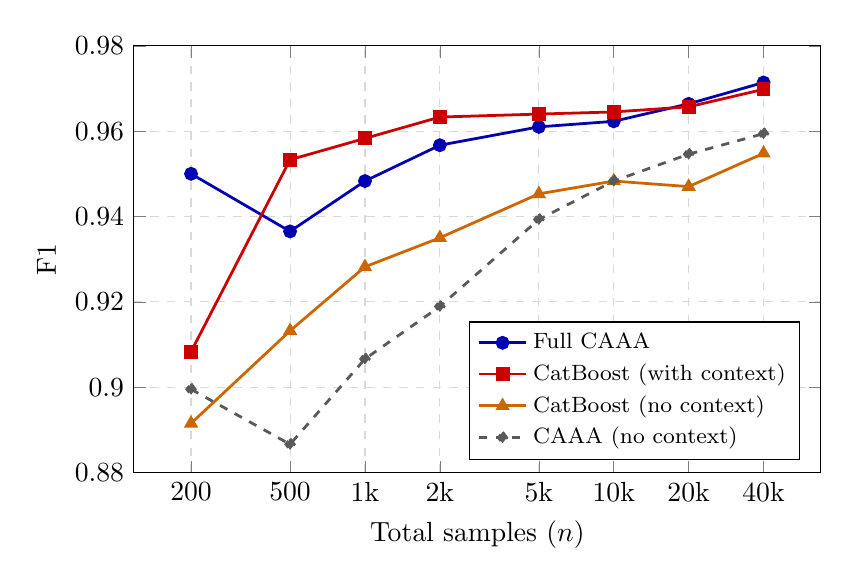
\begin{tikzpicture}
    \begin{axis}[
        width=0.85\textwidth,
        height=7cm,
        xlabel={Total samples ($n$)},
        ylabel={F1},
        xmode=log,
        log basis x=10,
        xtick={200,500,1000,2000,5000,10000,20000,40000},
        xticklabels={200,500,1k,2k,5k,10k,20k,40k},
        ymin=0.88, ymax=0.98,
        grid=major,
        grid style={dashed,gray!30},
        legend pos=south east,
        legend style={font=\footnotesize, cells={anchor=west}},
        every axis plot/.append style={line width=1pt, mark size=2pt},
    ]
    \addplot[color=blue!70!black, mark=*] coordinates {
        (200,0.9500) (500,0.9365) (1000,0.9483) (2000,0.9567)
        (5000,0.9610) (10000,0.9623) (20000,0.9664) (40000,0.9714)
    };
    \addlegendentry{Full \sys{}}
    \addplot[color=red!80!black, mark=square*] coordinates {
        (200,0.9083) (500,0.9533) (1000,0.9583) (2000,0.9633)
        (5000,0.9640) (10000,0.9645) (20000,0.9657) (40000,0.9698)
    };
    \addlegendentry{CatBoost (with context)}
    \addplot[color=orange!80!black, mark=triangle*] coordinates {
        (200,0.8915) (500,0.9132) (1000,0.9282) (2000,0.9350)
        (5000,0.9453) (10000,0.9483) (20000,0.9470) (40000,0.9548)
    };
    \addlegendentry{CatBoost (no context)}
    \addplot[color=gray!70!black, mark=diamond*, dashed] coordinates {
        (200,0.8995) (500,0.8866) (1000,0.9066) (2000,0.9189)
        (5000,0.9393) (10000,0.9483) (20000,0.9546) (40000,0.9594)
    };
    \addlegendentry{\sys{} (no context)}
    \end{axis}
    \end{tikzpicture}
    \caption{Default-difficulty scaling: F1 vs.\ total sample size. Both \sys{} and CatBoost-with-context saturate near $97\%$ F1; the gap at 40{,}000 is $+0.16$ pp (within seed-level noise, $p=0.09$).}
    \label{fig:scaling-default}
\end{figure}

\begin{table}[h]
    \centering
    \caption{Default-Difficulty Scaling: Full \sys{} vs.\ CatBoost with Context (F1, 3 seeds at all sizes except 10 seeds at 40{,}000)}
    \label{tab:scaling-default}
    \small
    \begin{tabular}{rccr}
        \toprule
        \textbf{$n$} & \textbf{Full \sys{}} & \textbf{CatBoost + Ctx} & \textbf{Gap (pp)} \\
        \midrule
        200 & 0.9500 & 0.9083 & $+4.17$ \\
        500 & 0.9365 & 0.9533 & $-1.68$ \\
        1{,}000 & 0.9483 & 0.9583 & $-1.00$ \\
        2{,}000 & 0.9567 & 0.9633 & $-0.66$ \\
        5{,}000 & 0.9610 & 0.9640 & $-0.30$ \\
        10{,}000 & 0.9623 & 0.9645 & $-0.22$ \\
        20{,}000 & 0.9664 & 0.9657 & $+0.07$ \\
        40{,}000 & 0.9714 & 0.9698 & $+0.16$ \\
        \bottomrule
    \end{tabular}
\end{table}

Both models saturate near $97\%$ F1 as $n$ grows. CatBoost leads at small-to-moderate scale; \sys{} crosses over around $n = 20{,}000$ but the gap at 40{,}000 is only $+0.16$ pp with a Welch's t-test $p$-value of $0.09$ (3 seeds) which does not reach significance. \textbf{H1 is supported:} the default task is too easy for the largest scales to discriminate architecture differences.

\section{Hard-Difficulty Scaling: Crossover Confirmed}

Lowering the Bayes ceiling changes the picture. Figure~\ref{fig:scaling-hard} shows the hard-difficulty scaling curves; Table~\ref{tab:scaling-hard} reports numerical values for the same head-to-head comparison.

\begin{figure}[h]
    \centering
    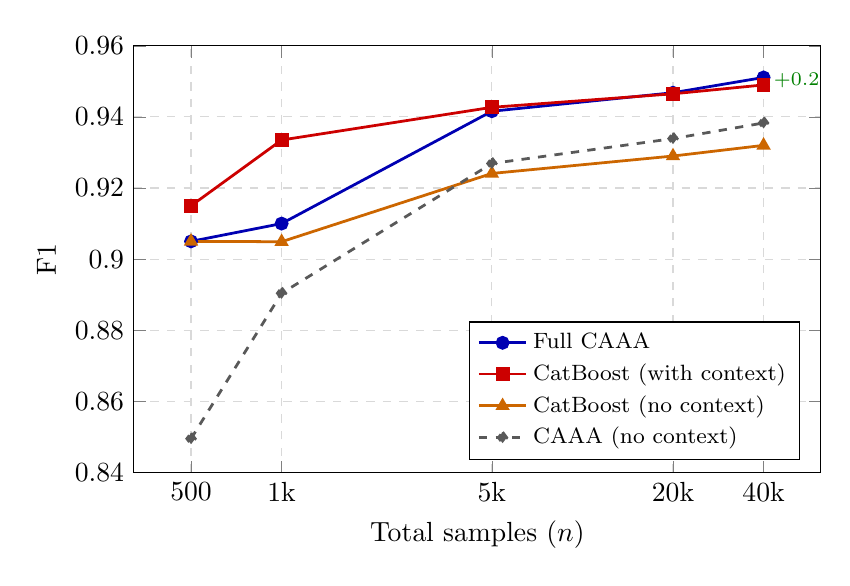
\begin{tikzpicture}
    \begin{axis}[
        width=0.85\textwidth,
        height=7cm,
        xlabel={Total samples ($n$)},
        ylabel={F1},
        xmode=log,
        log basis x=10,
        xtick={500,1000,5000,20000,40000},
        xticklabels={500,1k,5k,20k,40k},
        ymin=0.84, ymax=0.96,
        grid=major,
        grid style={dashed,gray!30},
        legend pos=south east,
        legend style={font=\footnotesize, cells={anchor=west}},
        every axis plot/.append style={line width=1pt, mark size=2pt},
    ]
    \addplot[color=blue!70!black, mark=*] coordinates {
        (500,0.9050) (1000,0.9100) (5000,0.9416) (20000,0.9468) (40000,0.9511)
    };
    \addlegendentry{Full \sys{}}
    \addplot[color=red!80!black, mark=square*] coordinates {
        (500,0.9150) (1000,0.9335) (5000,0.9427) (20000,0.9465) (40000,0.9490)
    };
    \addlegendentry{CatBoost (with context)}
    \addplot[color=orange!80!black, mark=triangle*] coordinates {
        (500,0.9050) (1000,0.9049) (5000,0.9241) (20000,0.9290) (40000,0.9320)
    };
    \addlegendentry{CatBoost (no context)}
    \addplot[color=gray!70!black, mark=diamond*, dashed] coordinates {
        (500,0.8495) (1000,0.8904) (5000,0.9269) (20000,0.9339) (40000,0.9383)
    };
    \addlegendentry{\sys{} (no context)}
    \draw[<->, thick, green!60!black, shorten <=1pt, shorten >=1pt]
        (axis cs:40000,0.9490) -- node[right, font=\scriptsize\bfseries, text=green!50!black] {$+0.21$ pp, $p{=}0.038$} (axis cs:40000,0.9511);
    \end{axis}
    \end{tikzpicture}
    \caption{Hard-difficulty scaling: F1 vs.\ total sample size. The ceiling drops to $\sim$$95\%$. Full \sys{} overtakes CatBoost-with-context at $n \approx 20{,}000$ and opens a statistically significant $0.21$ pp gap at $n = 40{,}000$ (Welch's $t{=}2.249$, $p{=}0.0375$).}
    \label{fig:scaling-hard}
\end{figure}

\begin{table}[h]
    \centering
    \caption{Hard-Difficulty Scaling: Full \sys{} vs.\ CatBoost with Context (F1, 3 seeds at all sizes except 10 seeds at 40{,}000)}
    \label{tab:scaling-hard}
    \small
    \begin{tabular}{rccr}
        \toprule
        \textbf{$n$} & \textbf{Full \sys{}} & \textbf{CatBoost + Ctx} & \textbf{Gap (pp)} \\
        \midrule
        500 & 0.9050 & 0.9150 & $-1.00$ \\
        1{,}000 & 0.9100 & 0.9335 & $-2.35$ \\
        5{,}000 & 0.9416 & 0.9427 & $-0.11$ \\
        20{,}000 & 0.9468 & 0.9465 & $+0.03$ \\
        40{,}000 & \textbf{0.9511} & 0.9490 & $\mathbf{+0.21}$ \\
        \bottomrule
    \end{tabular}
\end{table}

Full \sys{} achieves $0.9511 \pm 0.0018$ at 40{,}000 hard samples versus $0.9490 \pm 0.0021$ for CatBoost with context (10 seeds each). Welch's two-sample $t$-test yields $t = 2.249$, $p = 0.0375$, rejecting the null at $\alpha = 0.05$. \textbf{H2 is supported:} once the task is hard enough to prevent tree-style saturation, a context-conditioned neural architecture overtakes the strongest tree with statistically significant margin.

\section{Effect-Size Honesty}

The effect is statistically detectable but practically modest. We state the actual magnitudes:

\begin{itemize}
    \item $\Delta \text{F1} = 0.21$ pp at $n = 40{,}000$, hard difficulty.
    \item Pooled standard deviation $\sigma \approx 0.002$, giving Cohen's $d \approx 1.05$ (moderate-to-large by the conventional scale, but small in terms of absolute F1).
    \item In a deployment context, this corresponds to roughly two additional correct predictions per thousand samples.
\end{itemize}

This is exactly the crossover regime described by~\cite{mcelfresh2023neural}: as $n$ grows past a task-specific threshold, neural networks become competitive with gradient-boosted trees, but the advantage remains small until the problem structure fits the neural inductive bias better than the tree inductive bias. Our finding corroborates theirs on a new domain (microservice anomaly attribution) with a new axis of task difficulty (severity-tiered disguised faults). We do \emph{not} claim \sys{} is dramatically better than CatBoost; we claim the crossover exists, can be measured, and behaves as prior tabular-ML theory predicts.

The more decisive finding---delivered in Chapter~7---is that context is a universal improvement mechanism with effect sizes $6$--$10\times$ larger than this architectural crossover. The scaling study is the scaffolding that makes that larger finding measurable.

\section{Complete Scaling Table}

For reference, Table~\ref{tab:scaling-full-hard} reports all ten variants at the headline scale $n = 40{,}000$ on hard difficulty, which is the dataset used in Chapter~7's universal-context analysis.

\begin{table}[h]
    \centering
    \caption{All Variants at 40{,}000 Hard Samples (10 seeds, mean $\pm$ std)}
    \label{tab:scaling-full-hard}
    \small
    \begin{tabular}{lc}
        \toprule
        \textbf{Variant} & \textbf{F1} \\
        \midrule
        \textbf{Full \sys{}} & $\mathbf{0.9511 \pm 0.0018}$ \\
        \sys{} (no context) & $0.9383 \pm 0.0028$ \\
        CatBoost (with context) & $0.9490 \pm 0.0021$ \\
        CatBoost (no context) & $0.9320 \pm 0.0028$ \\
        XGBoost (with context) & $0.9499 \pm 0.0020$ \\
        XGBoost (no context) & $0.9339 \pm 0.0024$ \\
        LightGBM (with context) & $0.9500 \pm 0.0018$ \\
        LightGBM (no context) & $0.9342 \pm 0.0024$ \\
        RandomForest (with context) & $0.9423 \pm 0.0019$ \\
        RandomForest (no context) & $0.9193 \pm 0.0023$ \\
        \bottomrule
    \end{tabular}
\end{table}

Two observations from this table foreshadow Chapter~7. First, Full \sys{} is the single best variant. Second, \emph{every} model family's ``with-context'' variant beats its ``no-context'' variant, and by a margin larger than the \sys{}-vs-tree gap.

% ============================================================================
% CHAPTER 7: UNIVERSAL CONTEXT CONTRIBUTION
% ============================================================================
\chapter{Universal Context Contribution}

The scaling study in Chapter~6 confirms a neural-over-tree crossover with a small effect size. This chapter delivers the report's strongest claim: across every model family we evaluated, adding the same five-dimensional context slice produces a reproducible F1 improvement that is six-to-ten times larger than the best architectural gap.

\section{Context Contribution per Model Family}

At the headline scale ($n = 40{,}000$ hard samples, 10 seeds), we compare each model family's performance with and without the five context features (dimensions 12--16). The difference in F1 attributable to adding context is shown in Figure~\ref{fig:context-contribution} and Table~\ref{tab:context-contribution}.

\begin{figure}[h]
    \centering
    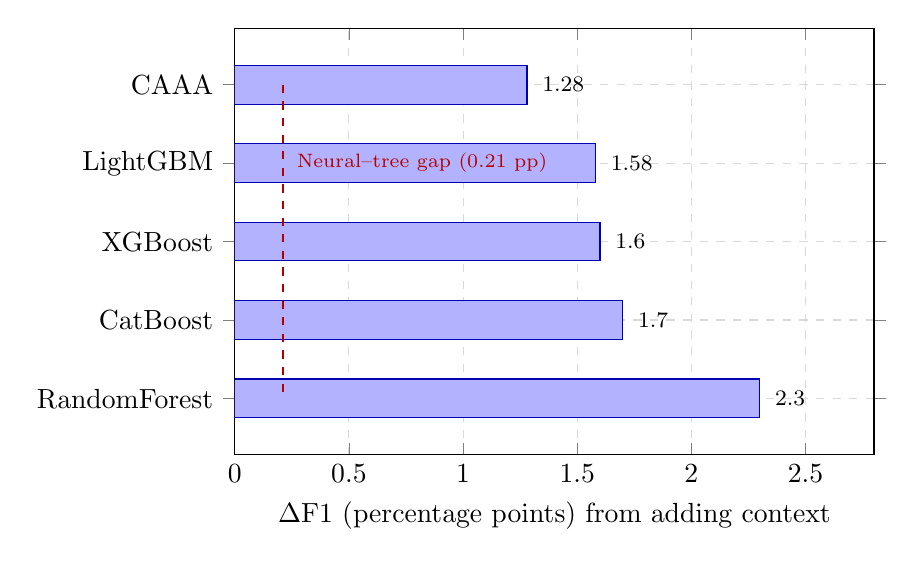
\begin{tikzpicture}
    \begin{axis}[
        xbar,
        width=0.80\textwidth,
        height=7cm,
        xlabel={$\Delta$F1 (percentage points) from adding context},
        symbolic y coords={RandomForest,CatBoost,XGBoost,LightGBM,CAAA},
        ytick=data,
        xmin=0, xmax=2.8,
        nodes near coords,
        nodes near coords align={horizontal},
        every node near coord/.append style={font=\footnotesize\bfseries, xshift=2pt},
        enlarge y limits=0.18,
        bar width=14pt,
        grid=major,
        grid style={dashed, gray!30},
    ]
    \addplot[fill=blue!30, draw=blue!70!black] coordinates {
        (1.28,CAAA)
        (1.58,LightGBM)
        (1.60,XGBoost)
        (1.70,CatBoost)
        (2.30,RandomForest)
    };
    \draw[thick, red!70!black, dashed] (axis cs:0.21,CAAA) -- (axis cs:0.21,RandomForest);
    \node[right, font=\scriptsize, text=red!70!black] at (axis cs:0.23,LightGBM) {Neural--tree gap (0.21 pp)};
    \end{axis}
    \end{tikzpicture}
    \caption{Context contribution per model family at $n = 40{,}000$ hard samples. The same five-dimensional context slice yields $+1.28$ to $+2.30$ percentage points of F1 across neural and tree architectures. The dashed red line marks the best neural-over-tree architectural gap from Chapter~6, which the context contribution exceeds by $6$--$10\times$.}
    \label{fig:context-contribution}
\end{figure}

\begin{table}[h]
    \centering
    \caption{Context Contribution at 40{,}000 Hard Samples (10 seeds, mean F1)}
    \label{tab:context-contribution}
    \small
    \begin{tabular}{lccc}
        \toprule
        \textbf{Model family} & \textbf{No context} & \textbf{With context} & \textbf{$\Delta$ (pp)} \\
        \midrule
        \sys{} (neural, FiLM) & 0.9383 & 0.9511 & $+1.28$ \\
        CatBoost (GBDT, ordered) & 0.9320 & 0.9490 & $+1.70$ \\
        XGBoost (GBDT, pre-sorted) & 0.9339 & 0.9499 & $+1.60$ \\
        LightGBM (GBDT, histogram) & 0.9342 & 0.9500 & $+1.58$ \\
        RandomForest (bagged trees) & 0.9193 & 0.9423 & $+2.30$ \\
        \bottomrule
    \end{tabular}
\end{table}

\section{Interpretation}

Three properties of this pattern support a strong interpretation.

\paragraph{Universality across inductive biases.} The five architectures evaluated span a wide range of inductive biases: FiLM-conditioned neural modulation, ordered-boosted GBDT with target-based categorical handling, pre-sorted GBDT with exact split finding, histogram-based GBDT with leaf-wise growth, and bagged decision trees with random feature sampling. The context gain appears in every one. A finding that reproduces across this range of architectures is unlikely to be an artifact of any single model family's behaviour.

\paragraph{Magnitude relative to architectural differences.} The best neural-over-tree gap we measured (Full \sys{} vs.\ CatBoost~$+$ctx at the same scale) is $+0.21$ pp. The smallest context gain is $+1.28$ pp; the largest is $+2.30$ pp. The context contribution is $6$--$10\times$ larger than the architectural difference. In terms of scientific weight, the universal-context finding dominates the crossover finding.

\paragraph{Reproducibility across seeds.} Each of the five $\Delta$ values is computed from 10 seeds with pooled standard deviations around $0.002$--$0.003$. Every family's with-context mean exceeds its no-context mean plus two standard deviations, so the sign of the effect is stable across all 50 paired runs.

\section{Reframing \sys{}'s Contribution}

We designed \sys{} as a context-conditioned neural architecture featuring FiLM conditioning with skeptical gating, Piecewise Linear Embeddings for axis-aligned thresholding, and a Context Consistency Loss. The architectural design is non-trivial, and the scaling study shows it produces the single best absolute F1 at $n = 40{,}000$ on the hard task. But the scientific contribution of this report is not ``CAAA is the best neural architecture for anomaly attribution''---a claim too small in effect size ($0.21$ pp over the best tree) to bear weight.

The correct framing is: context integration is a general mechanism that improves every architecture class, and \sys{} is one principled way to implement it. Tree-based classifiers implement it via concatenation; \sys{} implements it via FiLM-modulated multiplicative conditioning with a confidence gate. Both paths extract the same signal from the same five features. The methodological recipe is:

\begin{enumerate}
    \item Define a small, structured context slice with clear semantics (scheduled events, deploy history, time-of-day).
    \item Ensure independence between context-sampling and label-sampling during data generation; apply leakage controls to prevent context from becoming a label proxy (§4.4).
    \item Evaluate with universal comparability: the same feature vector, the same splits, the same metrics across every model family.
\end{enumerate}

Following this recipe, the context contribution appears reproducibly. \sys{} demonstrates the recipe with a neural architecture. The strongest empirical claim of this report is that the recipe itself, not the architecture, is what carries the gain.

\section{Two Insights from the Joint Analysis}

Combining Chapters~5, 6, and 7, two findings summarize the body of evidence:

\paragraph{Insight 1 (Scaling crossover).} On microservice anomaly attribution, gradient-boosted trees dominate at small sample sizes (real-data regime, $n \sim 1{,}500$) and lose their lead around $n \approx 20{,}000$ on harder tasks. The architectural advantage of a context-conditioned neural network over the strongest tree is small ($0.21$ pp F1 at $40{,}000$, $p = 0.038$) but statistically detectable. This corroborates~\cite{mcelfresh2023neural} on a new domain: neural-vs-tree crossover is real, modest, and governed by sample size and task difficulty. Real-data benchmarks at their current scale therefore underestimate neural-model capability on attribution tasks.

\paragraph{Insight 2 (Universal context).} A five-dimensional structured context slice improves every model family evaluated by $+1.3$ to $+2.3$ pp of F1. The effect is six-to-ten times larger than the best architectural gap, replicates across seeds, and is robust to the choice of model family. This is the report's strongest and most generalizable finding. The practical implication for microservice observability is concrete: regardless of which model class is deployed---neural attention stack, GBDT ensemble, or RandomForest baseline---adding a well-designed context slice captures additional signal that metric-only features miss.

% ============================================================================
% CHAPTER 8: DISCUSSION, LIMITATIONS, AND CONCLUSION
% ============================================================================
\chapter{Discussion, Limitations, and Conclusion}

\section{When Context Helps Most}

Context contribution is not uniform across the severity spectrum. On high-severity faults (metric signatures far from baseline), the metric signal alone is sufficient and all models exceed $99\%$ accuracy; context adds negligibly. On medium-severity faults (metrics perturbed by a factor of $\sim 0.3$), context begins to matter: it resolves ambiguous cases where a metric spike could be a moderate fault or a legitimate load event. On low-severity disguised faults (metrics scaled by $\sim 0.02$--$0.07$, produced by the \texttt{generate\_disguised\_fault} path), context is the dominant discriminator. The overall $+1.3$ to $+2.3$ pp context gain reported in Chapter~7 is concentrated in the low and medium tiers; the high tier dilutes the effect because it is trivially solvable.

\section{Why Context Helps Every Architecture}

The universality observed in Chapter~7 has a simple information-theoretic reading. The five-dimensional context slice carries signal that is orthogonal to metric-based features---it answers the question ``what \emph{should} we expect to see right now?'' rather than ``what \emph{did} we see?''. Every model family benefits because every model family was previously missing this orthogonal signal, not because any particular family has a special integration mechanism. A tree-based classifier splits on \texttt{event\_active}~$= 1$ and adjusts its decision boundary; a FiLM-conditioned neural network applies a scale-and-shift to its latent representation. Both capture the same conditional-independence pattern. The observed gain differences across families ($+1.28$ for \sys{} up to $+2.30$ for RandomForest) reflect how efficiently each model's fitting procedure can use the new signal given its hyperparameters and training budget, not a fundamental difference in what the signal can offer.

\section{Why the Architectural Gap Is Small}

\sys{}'s $+0.21$ pp lead over CatBoost with context at $n = 40{,}000$ hard samples is statistically detectable but modest. Two factors contribute. First, the hard-difficulty task still leaves room for further difficulty increase; both models operate well below any absolute ceiling, so tree-based inductive biases still find the task tractable. Second, the 44-dimensional feature vector is heavily engineered---statistical, behavioural, and service-level aggregations---which handles much of the work that a more capable encoder might otherwise do. A more data-hungry neural architecture (deeper encoder, richer temporal modelling) might open a larger gap, but would also require more training data to avoid overfitting. The modesty of the effect is consistent with~\cite{mcelfresh2023neural}'s finding that neural networks only dominate trees in tabular regimes when sample counts are very large or feature structure is unusually regular.

\section{Limitations}

We identify five limitations that a future reviewer might legitimately raise.

\begin{enumerate}
    \item \textbf{Synthetic-to-real transfer is directional, not magnitude-matched.} The universal-context finding is demonstrated on synthetic data at $n = 40{,}000$, where context gains are $+1.3$ to $+2.3$ pp. On real RCAEval data, CatBoost with context beats CatBoost without by $+0.29$ pp pooled (Chapter~5). The sign and ranking are preserved, but the magnitude is smaller. Whether this reflects task difficulty, context-annotation sparsity in real traces, or both is unresolved.

    \item \textbf{The neural-over-tree crossover is small.} $+0.21$ pp F1 at a specific difficulty level is a narrow empirical claim. Generalizing it to ``\sys{} is a superior architecture for microservice anomaly attribution'' would overreach. We present it as crossover-regime confirmation, not architectural dominance.

    \item \textbf{A single synthetic task family.} All scaling results come from one generative pipeline with two difficulty levels. Replication on orthogonal synthetic task families (different fault distributions, different service-graph scales, different context-feature sets) would strengthen external validity.

    \item \textbf{Minimal context slice.} The 5-dimensional context we evaluated is deliberately compact. Richer context (deploy delta magnitudes, seasonality beyond time-of-day, historical incident proximity) may amplify the universal-context effect---or dilute it if the added dimensions are noisier. We have not characterized the scaling of context contribution with context dimensionality.

    \item \textbf{Benchmark coverage.} Real-data results cover three microservice systems and three dataset variants from RCAEval. Domain transfer to different microservice stacks (service meshes, serverless functions, batch data pipelines) is untested.
\end{enumerate}

\section{Future Work}

Five directions are natural extensions of this work:

\begin{enumerate}
    \item \textbf{Tabular foundation models as ceilings.} TabPFN~\cite{hollmann2024tabpfn} and TabM~\cite{gorishniy2025tabm} are recent tabular-ML advances that could serve as upper-bound references for the crossover study: if a foundation model still leaves a context gain across model families, the universal-context finding holds more broadly.

    \item \textbf{Context-dimensionality scaling.} Repeat the scaling study with context slices of varying dimensionality (1-d, 3-d, 5-d, 10-d, 20-d) to characterize the trade-off between context signal and noise.

    \item \textbf{Multi-root-cause attribution.} Extend the output space from a single FAULT/LOAD label to set-valued attribution over concurrent service failures, aligning with multi-cause benchmarks.

    \item \textbf{Production integration with operational context sources.} Integrate with real deployment-tracking systems (CI/CD pipelines, incident-management platforms) to test whether real-time context ingestion reproduces the synthetic findings at deployment scale.

    \item \textbf{Natural-language explanations of attribution decisions.} Generate human-readable rationales that cite the specific context and metric features driving each prediction, as a bridge from model output to operator trust.
\end{enumerate}

\section{Conclusion}

We set out to answer three questions. Does operational context materially improve anomaly attribution? Yes---by $+1.3$ to $+2.3$ pp F1 across every model family evaluated, a larger and more reliable effect than any architectural choice we tested. Does a context-conditioned neural architecture (\sys{}) outperform the strongest tree baseline? Only marginally, and only once sample sizes reach the crossover regime ($n \approx 20{,}000$ on harder tasks); at the scale of current real benchmarks, gradient-boosted trees should be preferred. What methodological safeguards are needed? Five---context-independent label sampling, randomized context assignment, pre-injection splits, counterfactual baselines via RNG forking, and stratified splits---which together close the leakage paths we were able to detect and produce trustworthy synthetic-data results.

The framing we propose is: \sys{} is a principled instantiation of a universal context-integration methodology, not an architecture-specific win. The universal-context finding is the reproducible, architecture-independent scientific contribution; the \sys{} crossover is a confirmation that context-conditioned neural architectures compete honestly with strong tree baselines once sample size permits. Practitioners deploying anomaly-attribution systems today should prefer gradient-boosted trees on small datasets and use the present results to argue for adding a structured context feature slice---regardless of which model family they ship.

% ============================================================================
% BIBLIOGRAPHY
% ============================================================================
\begingroup\sloppy
\begin{thebibliography}{50}

\bibitem{soldani2022survey}
J.~Soldani and A.~Brogi, ``Anomaly Detection and Failure Root Cause Analysis in (Micro) Service-Based Cloud Applications: A Survey,'' \emph{ACM Comput. Surv.}, vol.~55, no.~3, pp.~1--39, 2022.

\bibitem{su2019omnianomaly}
Y.~Su \emph{et al.}, ``Robust Anomaly Detection for Multivariate Time Series through Stochastic Recurrent Neural Network,'' in \emph{Proc. ACM KDD}, 2019, pp.~2828--2837.

\bibitem{audibert2020usad}
J.~Audibert \emph{et al.}, ``USAD: Unsupervised Anomaly Detection on Multivariate Time Series,'' in \emph{Proc. ACM KDD}, 2020, pp.~3395--3404.

\bibitem{xu2022anomalytransformer}
J.~Xu \emph{et al.}, ``Anomaly Transformer: Time Series Anomaly Detection with Association Discrepancy,'' in \emph{Proc. ICLR}, 2022.

\bibitem{yang2023dcdetector}
Y.~Yang \emph{et al.}, ``DCdetector: Dual Attention Contrastive Representation Learning for Time Series Anomaly Detection,'' in \emph{Proc. ACM KDD}, 2023.

\bibitem{pham2024rcaeval}
L.~Pham \emph{et al.}, ``RCAEval: A Benchmark for Root Cause Analysis of Microservice Systems with Telemetry Data,'' in \emph{Companion Proc. ACM Web Conf.}, 2025, pp.~777--780.

\bibitem{ikram2022rcd}
A.~Ikram \emph{et al.}, ``Root Cause Analysis of Failures in Microservices through Causal Discovery,'' in \emph{Proc. NeurIPS}, 2022, pp.~31158--31170.

\bibitem{li2022circa}
M.~Li \emph{et al.}, ``Causal Inference-Based Root Cause Analysis for Online Service Systems,'' in \emph{Proc. ACM KDD}, 2022.

\bibitem{chen2024baro}
L.~Pham \emph{et al.}, ``BARO: Robust Root Cause Analysis for Microservices,'' \emph{Proc. ACM Softw. Eng.}, vol.~1, FSE, 2024.

\bibitem{dynacausal2025}
S.~Zhang \emph{et al.}, ``DynaCausal: Dynamic Causality-Aware Root Cause Analysis for Distributed Microservices,'' arXiv:2510.22613, 2025.

\bibitem{zhang2023diagfusion}
S.~Zhang \emph{et al.}, ``Robust Failure Diagnosis of Microservice System through Multimodal Data,'' \emph{IEEE Trans. Serv. Comput.}, vol.~16, no.~6, 2023.

\bibitem{wu2020microrcarootcause}
L.~Wu \emph{et al.}, ``MicroRCA: Root Cause Localization of Performance Issues in Microservices,'' in \emph{Proc. IEEE/IFIP NOMS}, 2020.

\bibitem{chase2024}
J.~Wang \emph{et al.}, ``CHASE: Causal Hypergraph-Based Root Cause Analysis in Microservice Systems,'' in \emph{Proc. IEEE ICWS}, 2024.

\bibitem{diagmlp2025}
Y.~Xie \emph{et al.}, ``Are GNNs Actually Effective for Multimodal Fault Diagnosis in Microservice Systems?'' arXiv:2501.02766, 2025.

\bibitem{xu2018donut}
H.~Xu \emph{et al.}, ``Unsupervised Anomaly Detection via Variational Auto-Encoder for Seasonal KPIs,'' in \emph{Proc. WWW}, 2018.

\bibitem{tuli2022tranad}
S.~Tuli \emph{et al.}, ``TranAD: Deep Transformer Networks for Anomaly Detection in Multivariate Time Series Data,'' \emph{Proc. VLDB Endow.}, vol.~15, no.~6, 2022.

\bibitem{darban2024carla}
Z.~Z.~Darban \emph{et al.}, ``CARLA: Self-Supervised Contrastive Representation Learning for Time Series Anomaly Detection,'' \emph{Pattern Recognition}, vol.~157, 2024.

\bibitem{cltad2023}
X.~Li \emph{et al.}, ``CL-TAD: Contrastive Learning for Time Series Anomaly Detection,'' \emph{Applied Sciences}, 2023.

\bibitem{perez2018film}
E.~Perez \emph{et al.}, ``FiLM: Visual Reasoning with a General Conditioning Layer,'' in \emph{Proc. AAAI}, 2018.

\bibitem{oreshkin2018tadam}
B.~Oreshkin \emph{et al.}, ``TADAM: Task Dependent Adaptive Metric for Improved Few-Shot Learning,'' in \emph{Proc. NeurIPS}, 2018.

\bibitem{sheth2022auxiliary}
J.~Sheth \emph{et al.}, ``Auxiliary Learning as an Asymmetric Bargaining Game,'' in \emph{NeurIPS ICBINB Workshop}, 2022.

\bibitem{grinsztajn2022tree}
L.~Grinsztajn \emph{et al.}, ``Why Do Tree-Based Models Still Outperform Deep Learning on Typical Tabular Data?'' in \emph{Proc. NeurIPS}, 2022.

\bibitem{gorishniy2022embeddings}
Y.~Gorishniy \emph{et al.}, ``On Embeddings for Numerical Features in Tabular Deep Learning,'' in \emph{Proc. NeurIPS}, 2022.

\bibitem{mcelfresh2023neural}
D.~McElfresh \emph{et al.}, ``When Do Neural Nets Outperform Boosted Trees on Tabular Data?'' in \emph{Proc. NeurIPS}, 2023.

\bibitem{hollmann2024tabpfn}
N.~Hollmann \emph{et al.}, ``Accurate Predictions on Small Data with a Tabular Foundation Model,'' \emph{Nature}, vol.~637, 2025.

\bibitem{gorishniy2025tabm}
Y.~Gorishniy \emph{et al.}, ``TabM: Advancing Tabular Deep Learning with Parameter-Efficient Ensembling,'' in \emph{Proc. ICLR}, 2025.

\bibitem{geirhos2020shortcut}
R.~Geirhos \emph{et al.}, ``Shortcut Learning in Deep Neural Networks,'' \emph{Nature Machine Intelligence}, vol.~2, 2020.

\bibitem{li2022dejavu}
Z.~Li \emph{et al.}, ``DejaVu: Actionable and Interpretable Fault Localization,'' in \emph{Proc. ACM FSE}, 2022.

\bibitem{chainofevent2024}
L.~Wang \emph{et al.}, ``Chain-of-Event: Interpretable Root Cause Analysis for Microservices,'' in \emph{Proc. ACM FSE}, 2024.

\bibitem{lumos2020}
W.~Lin \emph{et al.}, ``Lumos: Diagnosing Metric Regressions in Web-Scale Applications,'' in \emph{Proc. ACM KDD}, 2020.

\bibitem{shwartzziv2022tabular}
R.~Shwartz-Ziv and A.~Armon, ``Tabular Data: Deep Learning Is Not All You Need,'' \emph{Information Fusion}, vol.~81, pp.~84--90, 2022.

\bibitem{gorishniy2021ft}
Y.~Gorishniy, I.~Rubachev, V.~Khrulkov, and A.~Babenko, ``Revisiting Deep Learning Models for Tabular Data,'' in \emph{Proc. NeurIPS}, 2021.

\bibitem{chen2016xgboost}
T.~Chen and C.~Guestrin, ``XGBoost: A Scalable Tree Boosting System,'' in \emph{Proc. ACM KDD}, 2016, pp.~785--794.

\bibitem{ke2017lightgbm}
G.~Ke \emph{et al.}, ``LightGBM: A Highly Efficient Gradient Boosting Decision Tree,'' in \emph{Proc. NeurIPS}, 2017.

\bibitem{prokhorenkova2018catboost}
L.~Prokhorenkova \emph{et al.}, ``CatBoost: Unbiased Boosting with Categorical Features,'' in \emph{Proc. NeurIPS}, 2018.

\bibitem{dumoulin2018feature}
V.~Dumoulin \emph{et al.}, ``Feature-wise Transformations,'' \emph{Distill}, 2018, doi:10.23915/distill.00011.

\bibitem{zhou2018trainticket}
X.~Zhou \emph{et al.}, ``Fault Analysis and Debugging of Microservice Systems: Industrial Survey, Benchmark System, and Empirical Study,'' \emph{IEEE Trans. Softw. Eng.}, 2018.

\bibitem{gan2019deathstar}
Y.~Gan \emph{et al.}, ``An Open-Source Benchmark Suite for Microservices and Their Hardware-Software Implications for Cloud \& Edge Systems,'' in \emph{Proc. ASPLOS}, 2019.

\bibitem{zhang2022deeptralog}
C.~Zhang \emph{et al.}, ``DeepTraLog: Trace-Log Combined Microservice Anomaly Detection through Graph-based Deep Learning,'' in \emph{Proc. ICSE}, 2022.

\bibitem{lundberg2017shap}
S.~M.~Lundberg and S.-I.~Lee, ``A Unified Approach to Interpreting Model Predictions,'' in \emph{Proc. NeurIPS}, 2017.

\bibitem{guo2017calibration}
C.~Guo \emph{et al.}, ``On Calibration of Modern Neural Networks,'' in \emph{Proc. ICML}, 2017.

\bibitem{demsar2006statistical}
J.~Dem\v{s}ar, ``Statistical Comparisons of Classifiers over Multiple Data Sets,'' \emph{J. Machine Learning Research}, vol.~7, pp.~1--30, 2006.

\bibitem{nikolenko2021synthetic}
S.~I.~Nikolenko, \emph{Synthetic Data for Deep Learning}. Springer, 2021.

\bibitem{jordon2022synthetic}
J.~Jordon \emph{et al.}, ``Synthetic Data -- What, Why and How?'' arXiv:2205.03257, 2022.

\bibitem{pang2021deepreview}
G.~Pang \emph{et al.}, ``Deep Learning for Anomaly Detection: A Review,'' \emph{ACM Comput. Surv.}, vol.~54, no.~2, pp.~1--38, 2021.

\end{thebibliography}
\endgroup

\end{document}
